\documentclass[a4paper,8pt]{extarticle}
\usepackage{graphicx}
\usepackage{extsizes}
\usepackage[a4paper, total={6in, 9in}]{geometry}
\usepackage[T1]{fontenc}
\usepackage[utf8]{inputenc}
\usepackage{graphicx}
\usepackage{tikz}
\usepackage{float}
\usepackage{mathtools}
\usepackage{fancyhdr}
\usepackage{caption}
\usepackage{textgreek}
\usepackage{yfonts}
\usepackage{amssymb}
\usepackage{hyperref}
\usepackage{amsmath}
\usepackage{systeme}
 \usepackage{subfig}
\hypersetup{
    colorlinks=true,
    linkcolor=blue,
    filecolor=magenta,
    urlcolor=cyan,
    pdftitle={Overleaf Example},
    pdfpagemode=FullScreen,
    }

\urlstyle{same}
\let\empty\varnothing
\let\eqv\Longleftrightarrow
\usepackage{longtable}
\graphicspath{./images}
\pagestyle{fancy}
\date{Março 2022}
\title{ \\ \large {Initial Report}}

\author{João Barreiros C. Rodrigues}

\begin{document}
        \pagenumbering{gobble}
        \begin{titlepage} % Suppresses displaying the page number on the title page and the subsequent page counts as page 1
        \newcommand{\HRule}{\rule{\linewidth}{0.5mm}} % Defines a new command for horizontal lines, change thickness here
        \center % Centre everything on the page
        \textsc{\LARGE Instituto Superior Técnico}\\[0.5cm] % Main heading such as the name of your university/college
       \textsc{\Large Bachelor's Degree in Electrical and Computer Engineering}\\[0.5cm] 
        \textsc{\Large Automatic Control}\\[0.25cm]
        \HRule\\[0.4cm]
        {\LARGE\bfseries Lab Report}\\[0.4cm] % Title of your document
        {\huge\bfseries Speed Control of a DC Motor}\\[0.4cm] % Title of your document
        \HRule\\[1.5cm]\
        João \textsc{Fortunato}, nº 96239 \\ 
        Nuno \textsc{Baptista}, nº 96295 \\
        João \textsc{Barreiros C. Rodrigues}, nº 99968 \\
        Group 121
        
        \vfill\vfill\vfill % Position the date 3/4 down the remaining page
        {\large June 2022} % Date, change the \today to a set date if you want to be precise
        \vfill % Push the date up 1/4 of the remaining page
\end{titlepage}
        \pagenumbering{arabic}
        \clearpage
        \section{Introduction}
        The goal of this laboratory assignment is to model, simulate, identify, and develop a feedback controller for the speed of a DC motor with a load gear, and also to enable us to grow our understand and insight of Control Theory and its applications.

        \section{Theoretical Notions and Deductions}
        
        \subsection*{Question 2.1}
        Applying the Laplace transform to equation (3) from the guide, we obtain:
        \begin{equation}
             Js\omega(s) = -b\omega(s) + K_{n}I(s)
        \end{equation}
        Solving equation (2) (also from the guide) for I, we find:
         \begin{equation}
             Js\omega(s) = -b\omega(s) + K_{n}[ \frac{V(s) - K_{e}\omega(s)}{R}]
        \end{equation}
        Finally, we solve equation (2) in order to obtain the transfer function:
         \begin{equation}
             G(s) = \frac{\Omega(s)}{V(s)} = \frac{K_{n}}{JRs + bR + K_{n}K_{e}}
        \end{equation}
        Rewriting equation (3), to obtain the expressions of k0 and a, we get:
        \begin{equation}
             G(s) = \frac{\Omega(s)}{V(s)} = k0\frac{a}{s+a} , with   
             \begin{cases}
             a = \frac{K_{n}K_{e} + bR}{RJ} \\
             k0 = \frac{K_{n}}{K_{n}K_{e} + bR}
             \end{cases}
        \end{equation}
        
        \subsection*{Question 3.1}
        In this question, we want to get the step response of G(s), in the time domain. In question 2.1, we got G(s), as shown in equation (3). We also know that the Laplace transform of the step response is:
         \begin{equation}
             \mathcal{L}\{u(t)\} = \frac{1}{s} 
        \end{equation}
        Applying the reverse Laplace transform to G(s), and solving the equation, we obtain:
         \begin{equation}
             \omega(s) = k0\frac{a}{s+a}V(s) = k0\frac{a}{s+a}\frac{1}{s} = k0\frac{a}{s^2+as} = k0[\frac{1}{s} - \frac{1}{s+a}]
        \end{equation}
        With same procedure, we find the step response of G(s):
          \begin{equation}
             \mathcal{L}^{-1}\{\omega(s)\} = k0[u(t) - e^{-at}] = k0[1 - e^{-at}]
        \end{equation}
        It is also requested the steady-state response, calculated below:
        \begin{equation}
             \begin{cases}
             w(t\to\infty) = k0 \\
             w(t = \frac{1}{a}) = k0(1-e^{\frac{-a}{a}}) = k0(1-e^{-1}) \simeq 0.632\cdot k0
             \end{cases}
        \end{equation}
        \clearpage
        \subsection*{Question 3.2}
           Analyzing the given equation of $G(s)$:\\
           \begin{equation}
               G(s)=k_0 \frac{a}{s+a}\text{, } k_0 > 0
           \end{equation}
            its easily deductible that the pole-zero plot has a pole located in -$a$ and no zeros, therefore the corresponding asymptotic Bode plot of the system must be similar to:\\
            \begin{figure}[H]
            \centering
            \captionsetup{justification=centering,margin=2cm}
            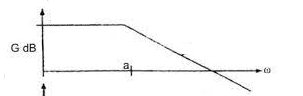
\includegraphics[width=0.4\textwidth]{asym_bode.jpg} 
            \caption{Asymptotic approximation of the system's transfer function Bode plot for amplitude}
            \\ This also allows us to infer that the cutoff frequency must be around $a$ Hz.
        \end{figure}
        \subsection*{Question 4.1}
        Using Matlab's ControlSystemDesigner feature, we were able to arbitrarily change the values of $k_{1}$ and $z$ so that the closed-loop transfer function meets the requirements. For the values of $k_{1}$ = 4 and $z$ = 67, the system satisfies all required design requisites, as shown below:
        \begin{figure}[H]
            \centering
            \captionsetup{justification=centering,margin=2cm}
            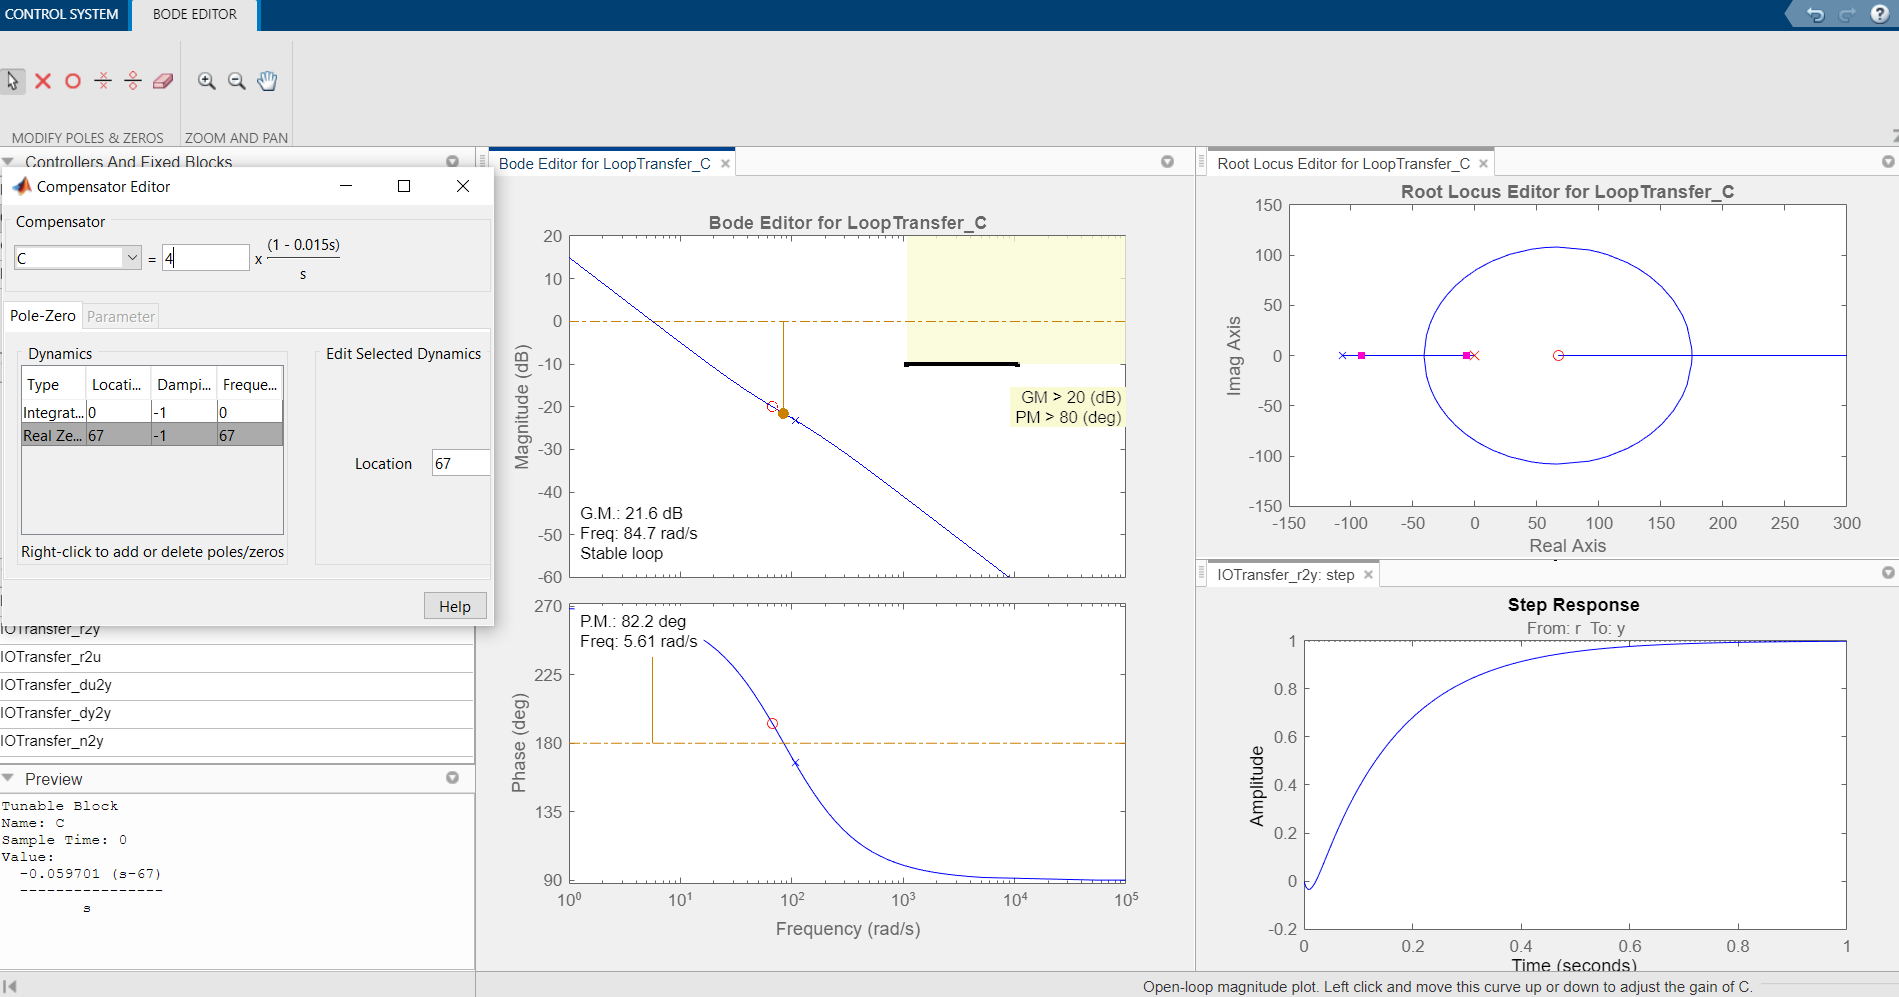
\includegraphics[width=9cm,height=5cm]{Screenshot (344).png} 
            \caption{Bode diagram, root locus and unit-step response for the simulated system when $k_{1}$ = 4 and $z$ = 67}
        \end{figure}
        With $z$ fixed at 67, the upper bound of $k_{1}$ so that the positive gain margin is equal or greater than 20 dB and the phase margin greater or equal than 80 degrees is 4.7996. 
        \subsection*{Question 4.2}
        According to Parseval's theorem:
        \begin{equation}
        \text{Energy of a signal }= \frac{1}{2\pi}\int_{-\infty}^{\infty}
        |X(j\omega)|^2 \,d\omega
        \end{equation}
        
        We need to make sure that for high frequencies the gain is bounded by a negative value in decibels, which means that the linear value of the gain is less than 1, so that the above integral is not infinite.
        \clearpage
        \subsection*{Question 4.3}
        First, we can assume that $\tau_{max}$ is given by the following relation:\\
        \begin{equation}
            \tau_{max}=\frac{\text{Phase Margin}}{\omega_{crossover}}
        \end{equation}
        By making the values of $k_{1}$ and $z$  above constant, we found that the maximum value of $\tau$ that the system can tolerate without going unstable is 0.25 seconds. When such a time delay happens, both the gain and phase margin decrease, to 0.2 dB and 72 degrees, respectively.
        \begin{figure}[H]
            \centering
            \captionsetup{justification=centering,margin=2cm}
            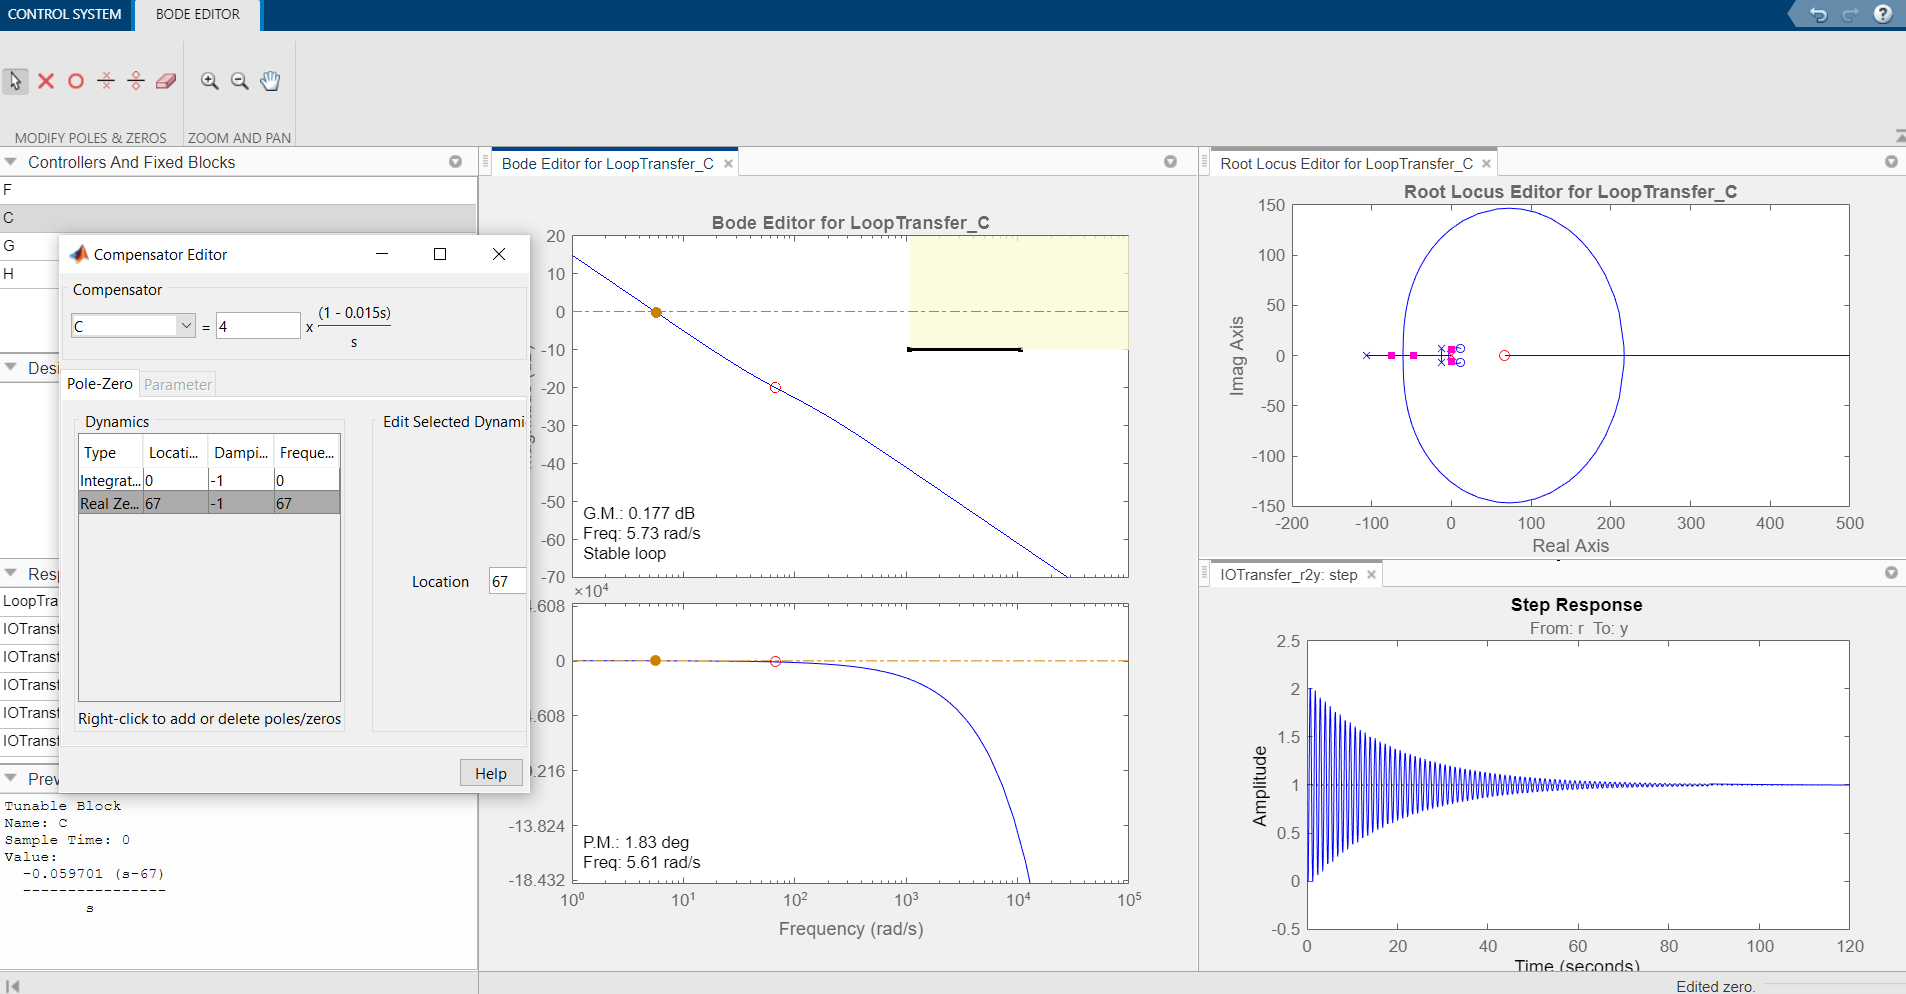
\includegraphics[width=15cm,height=8cm]{Screenshot (345).png} 
            \caption{Characteristics of the closed-loop system when there is a time delay of 0.25 seconds between the controller and the system.}
        \end{figure}
        It is important to observe that in the situation described above not only both the gain margin and phase margin are greatly reduced, but the system also becomes highly oscillating, however it still stabilizes, since it tends to 1 in infinity.
        \clearpage
        
    \section{Laboratorial Observations}
         \subsection*{Question 3.3}
          In order to find $k_{0}$ and $a$, a direct comparison procedure was followed: \\
          Initially we set $a$ to 5 and varied $k_0$ until the computed experimental static gain roughly coincided with the plotted theoretical static gain.\\
          Then with $k_0$ determined ($k_0$ = 1.4), using the relation obtained in equation (4) a rough estimate of $a$ was determined, allowing finer tuning with a scrapping of decimal values.\\
          We present a photographic summary of the procedure below:
          \begin{figure}[ht]
            \centering
            \captionsetup{justification=centering}
            \subfloat[\centering]{{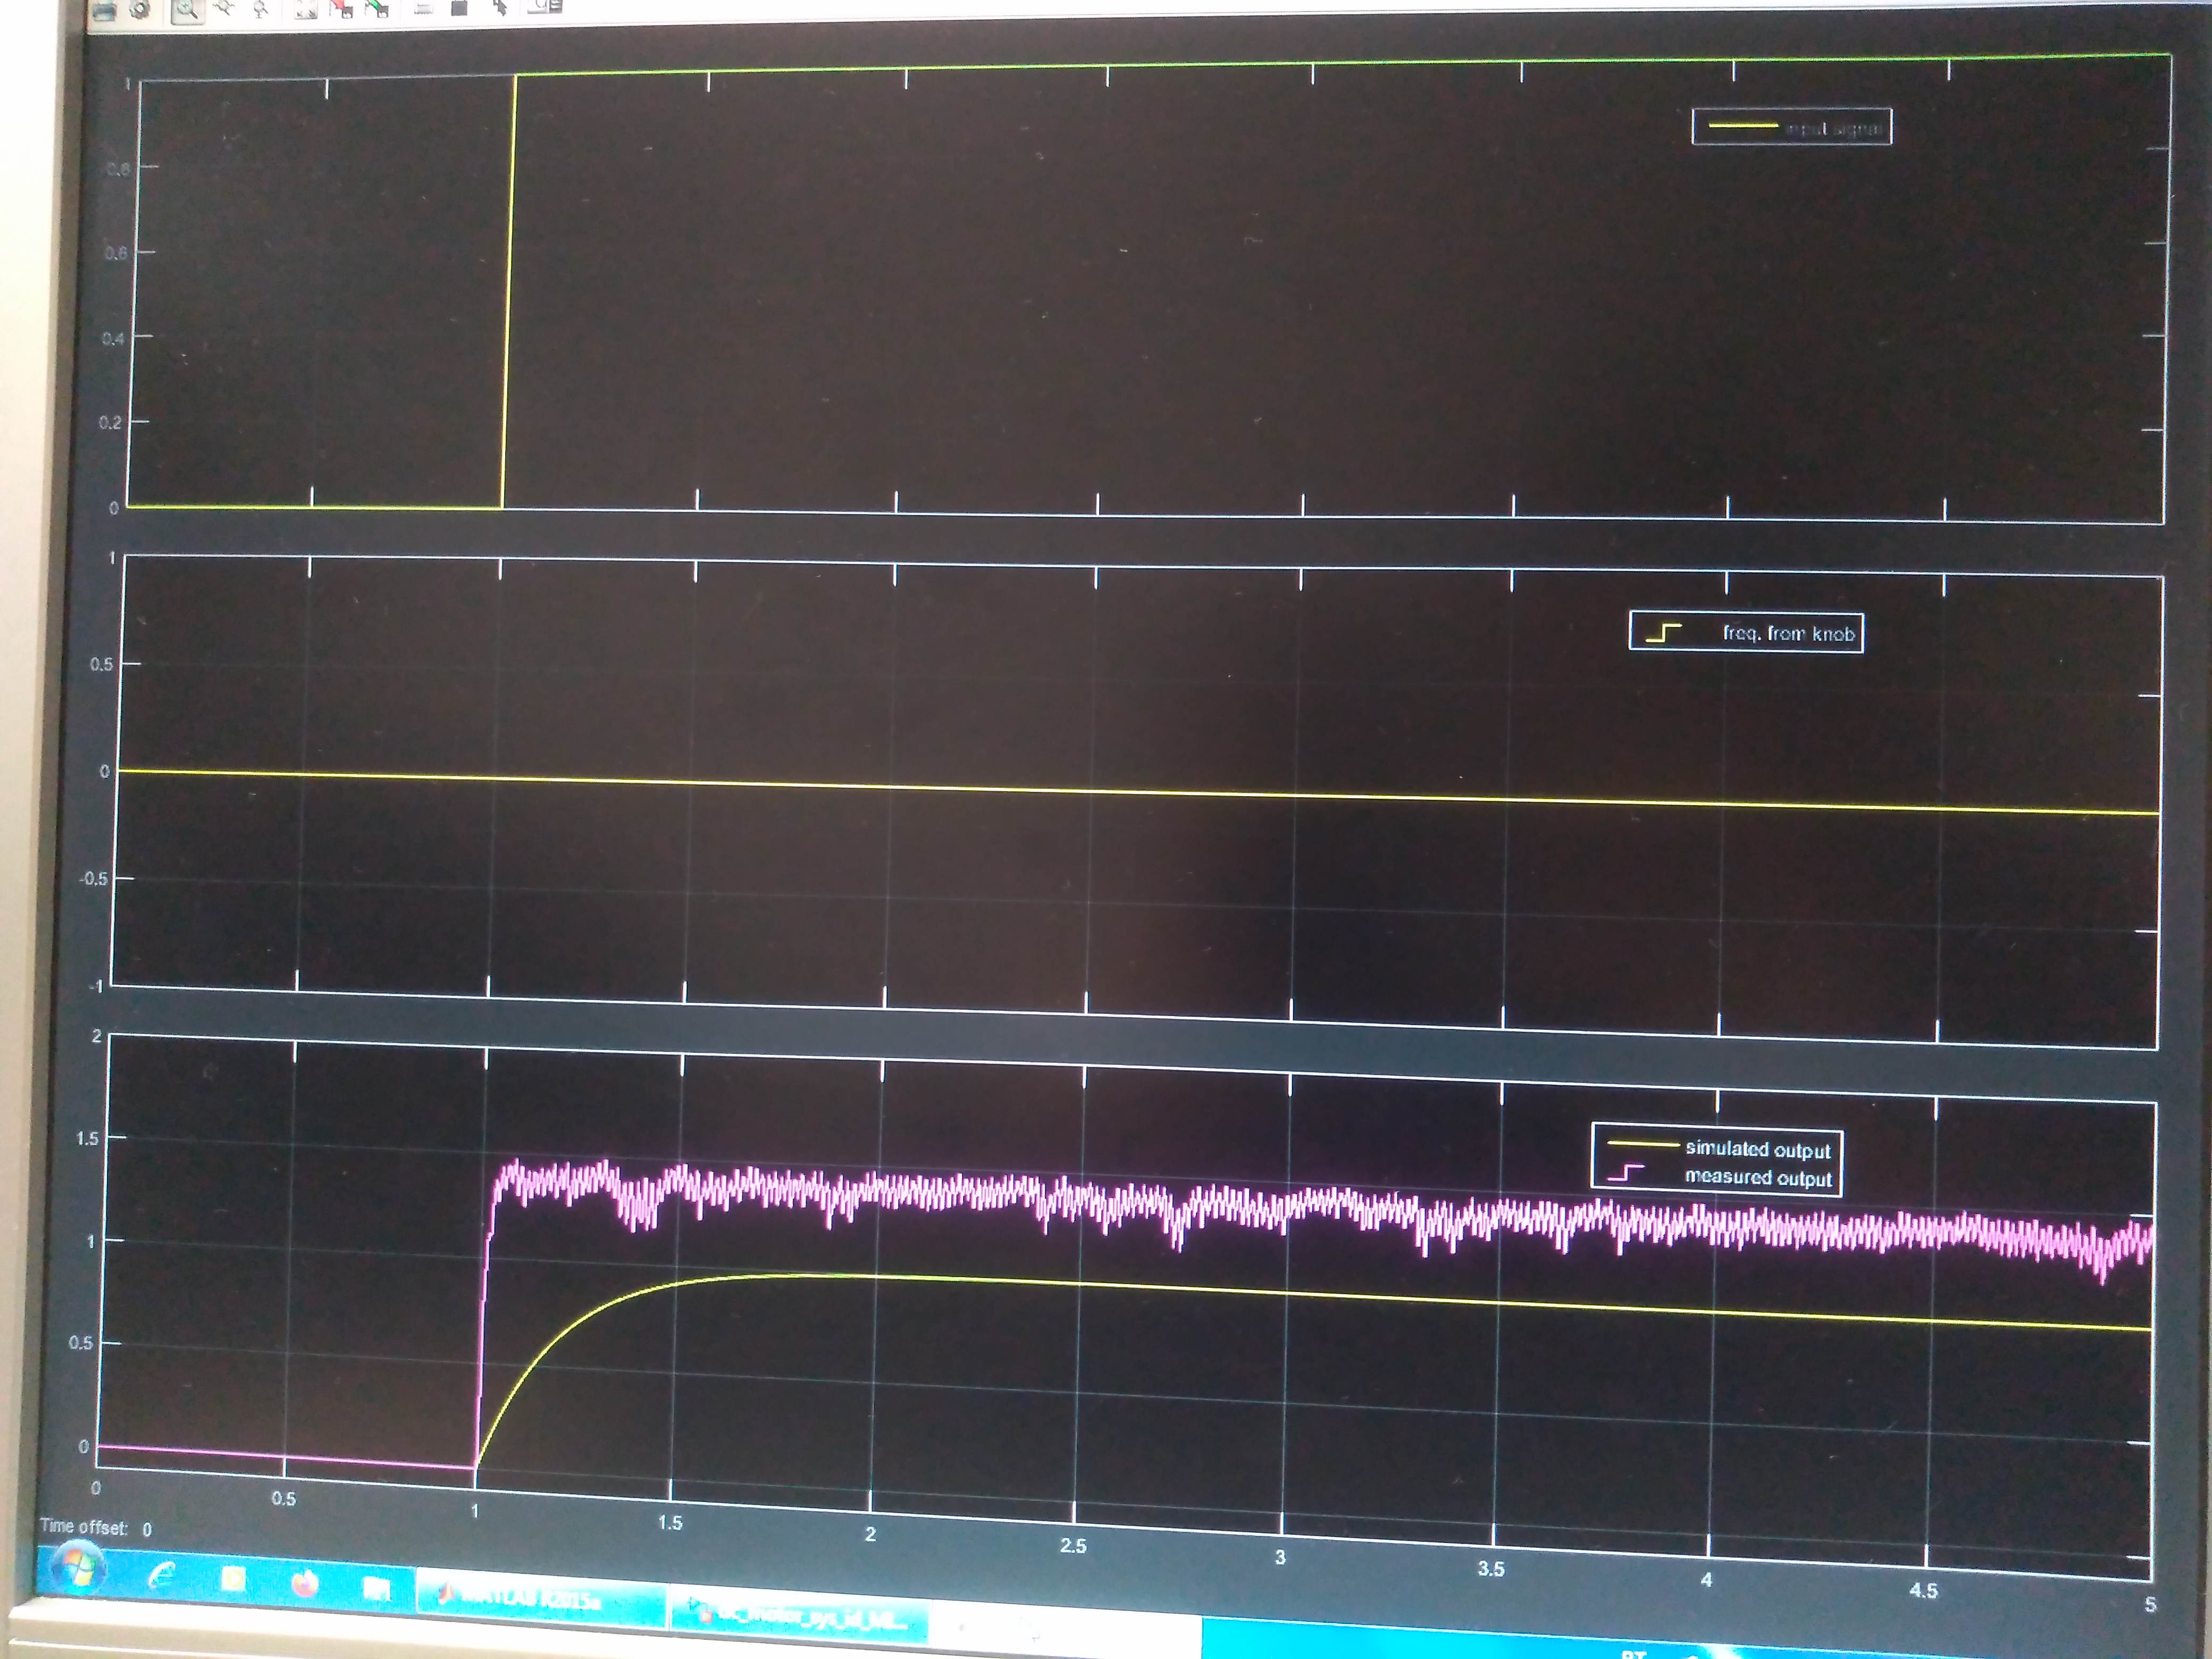
\includegraphics[width=7cm]{k0_1.jpg}}}%
            \qquad
            \subfloat[\centering]{{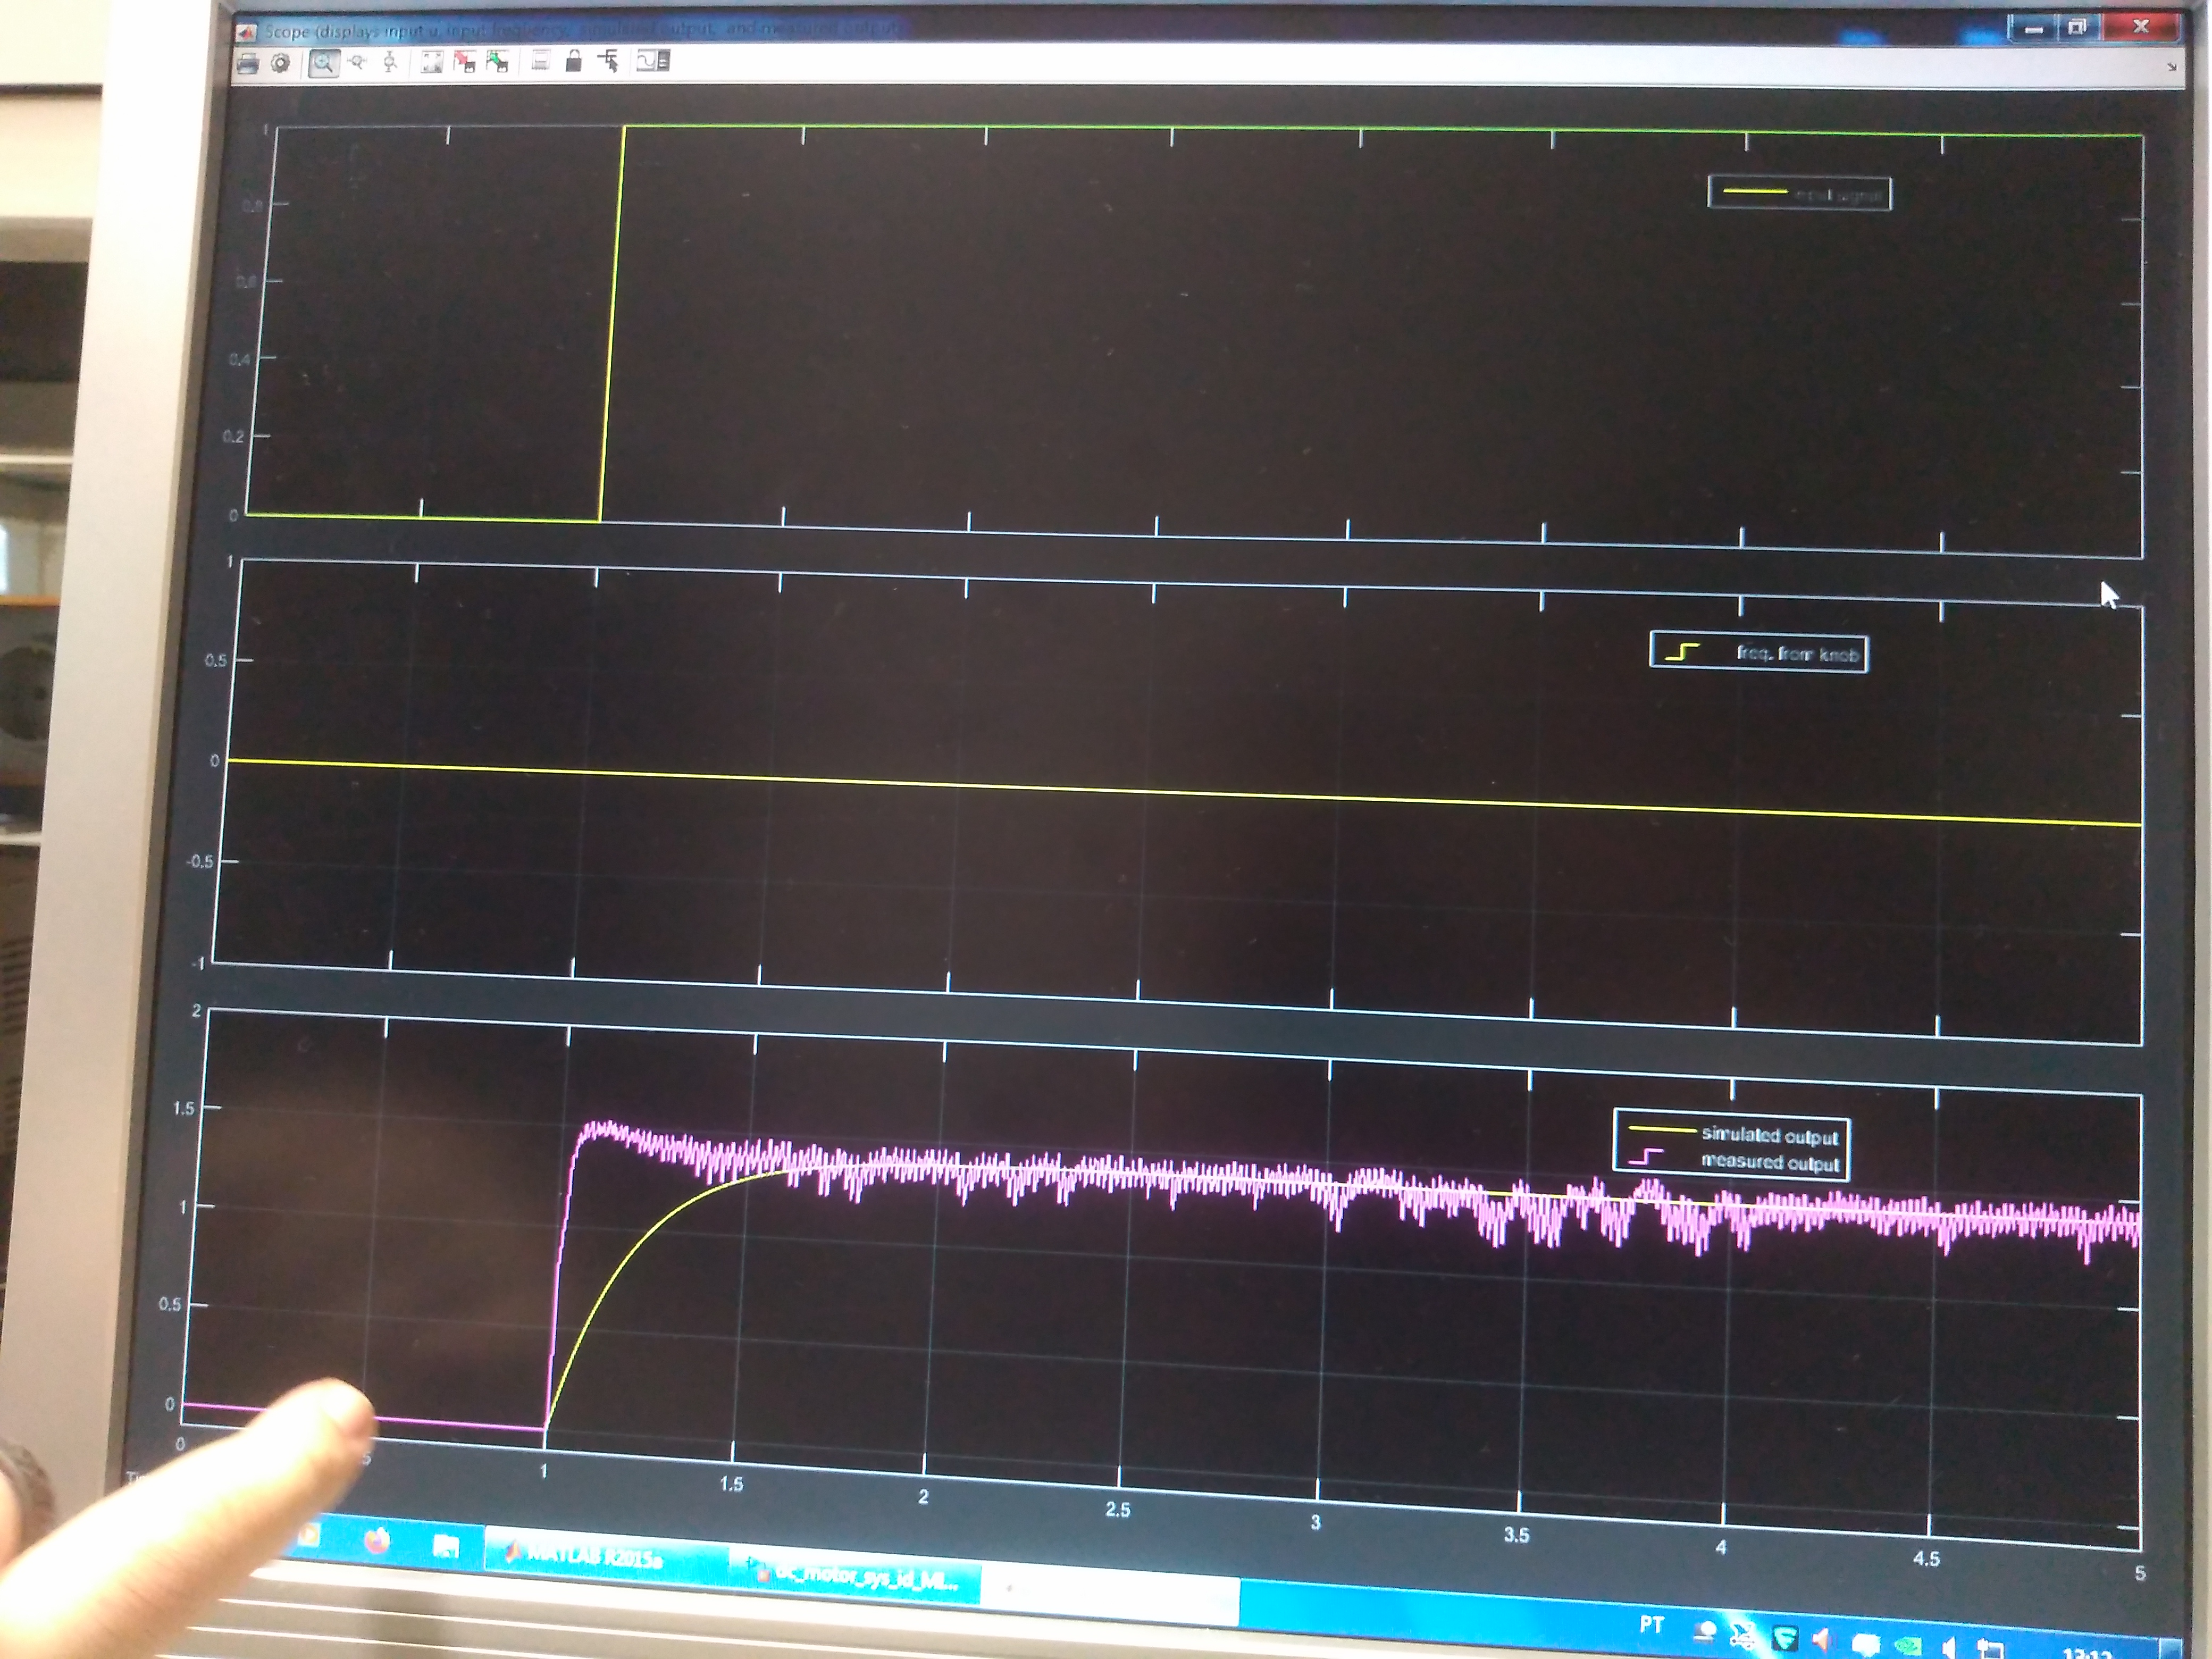
\includegraphics[width=7cm]{k01_4_a_5.jpg}}}%
        \caption{Pictured left and right, the system response plot for both simulated (yellow) and experimental (pink) situations for $k_0$=1 and $k_0$=1.4, respectively}
        \end{figure}
        \\ In addition, a system response plot for $k_0$=1.5 (not pictured) was obtained after plot (a), which had a experimental static gain inferior to the theoretical, which motivated us to experiment with $k_0$=1.4 (b)
         \begin{figure}[ht]
         \centering
            \captionsetup{justification=centering}
            \subfloat[\centering]{{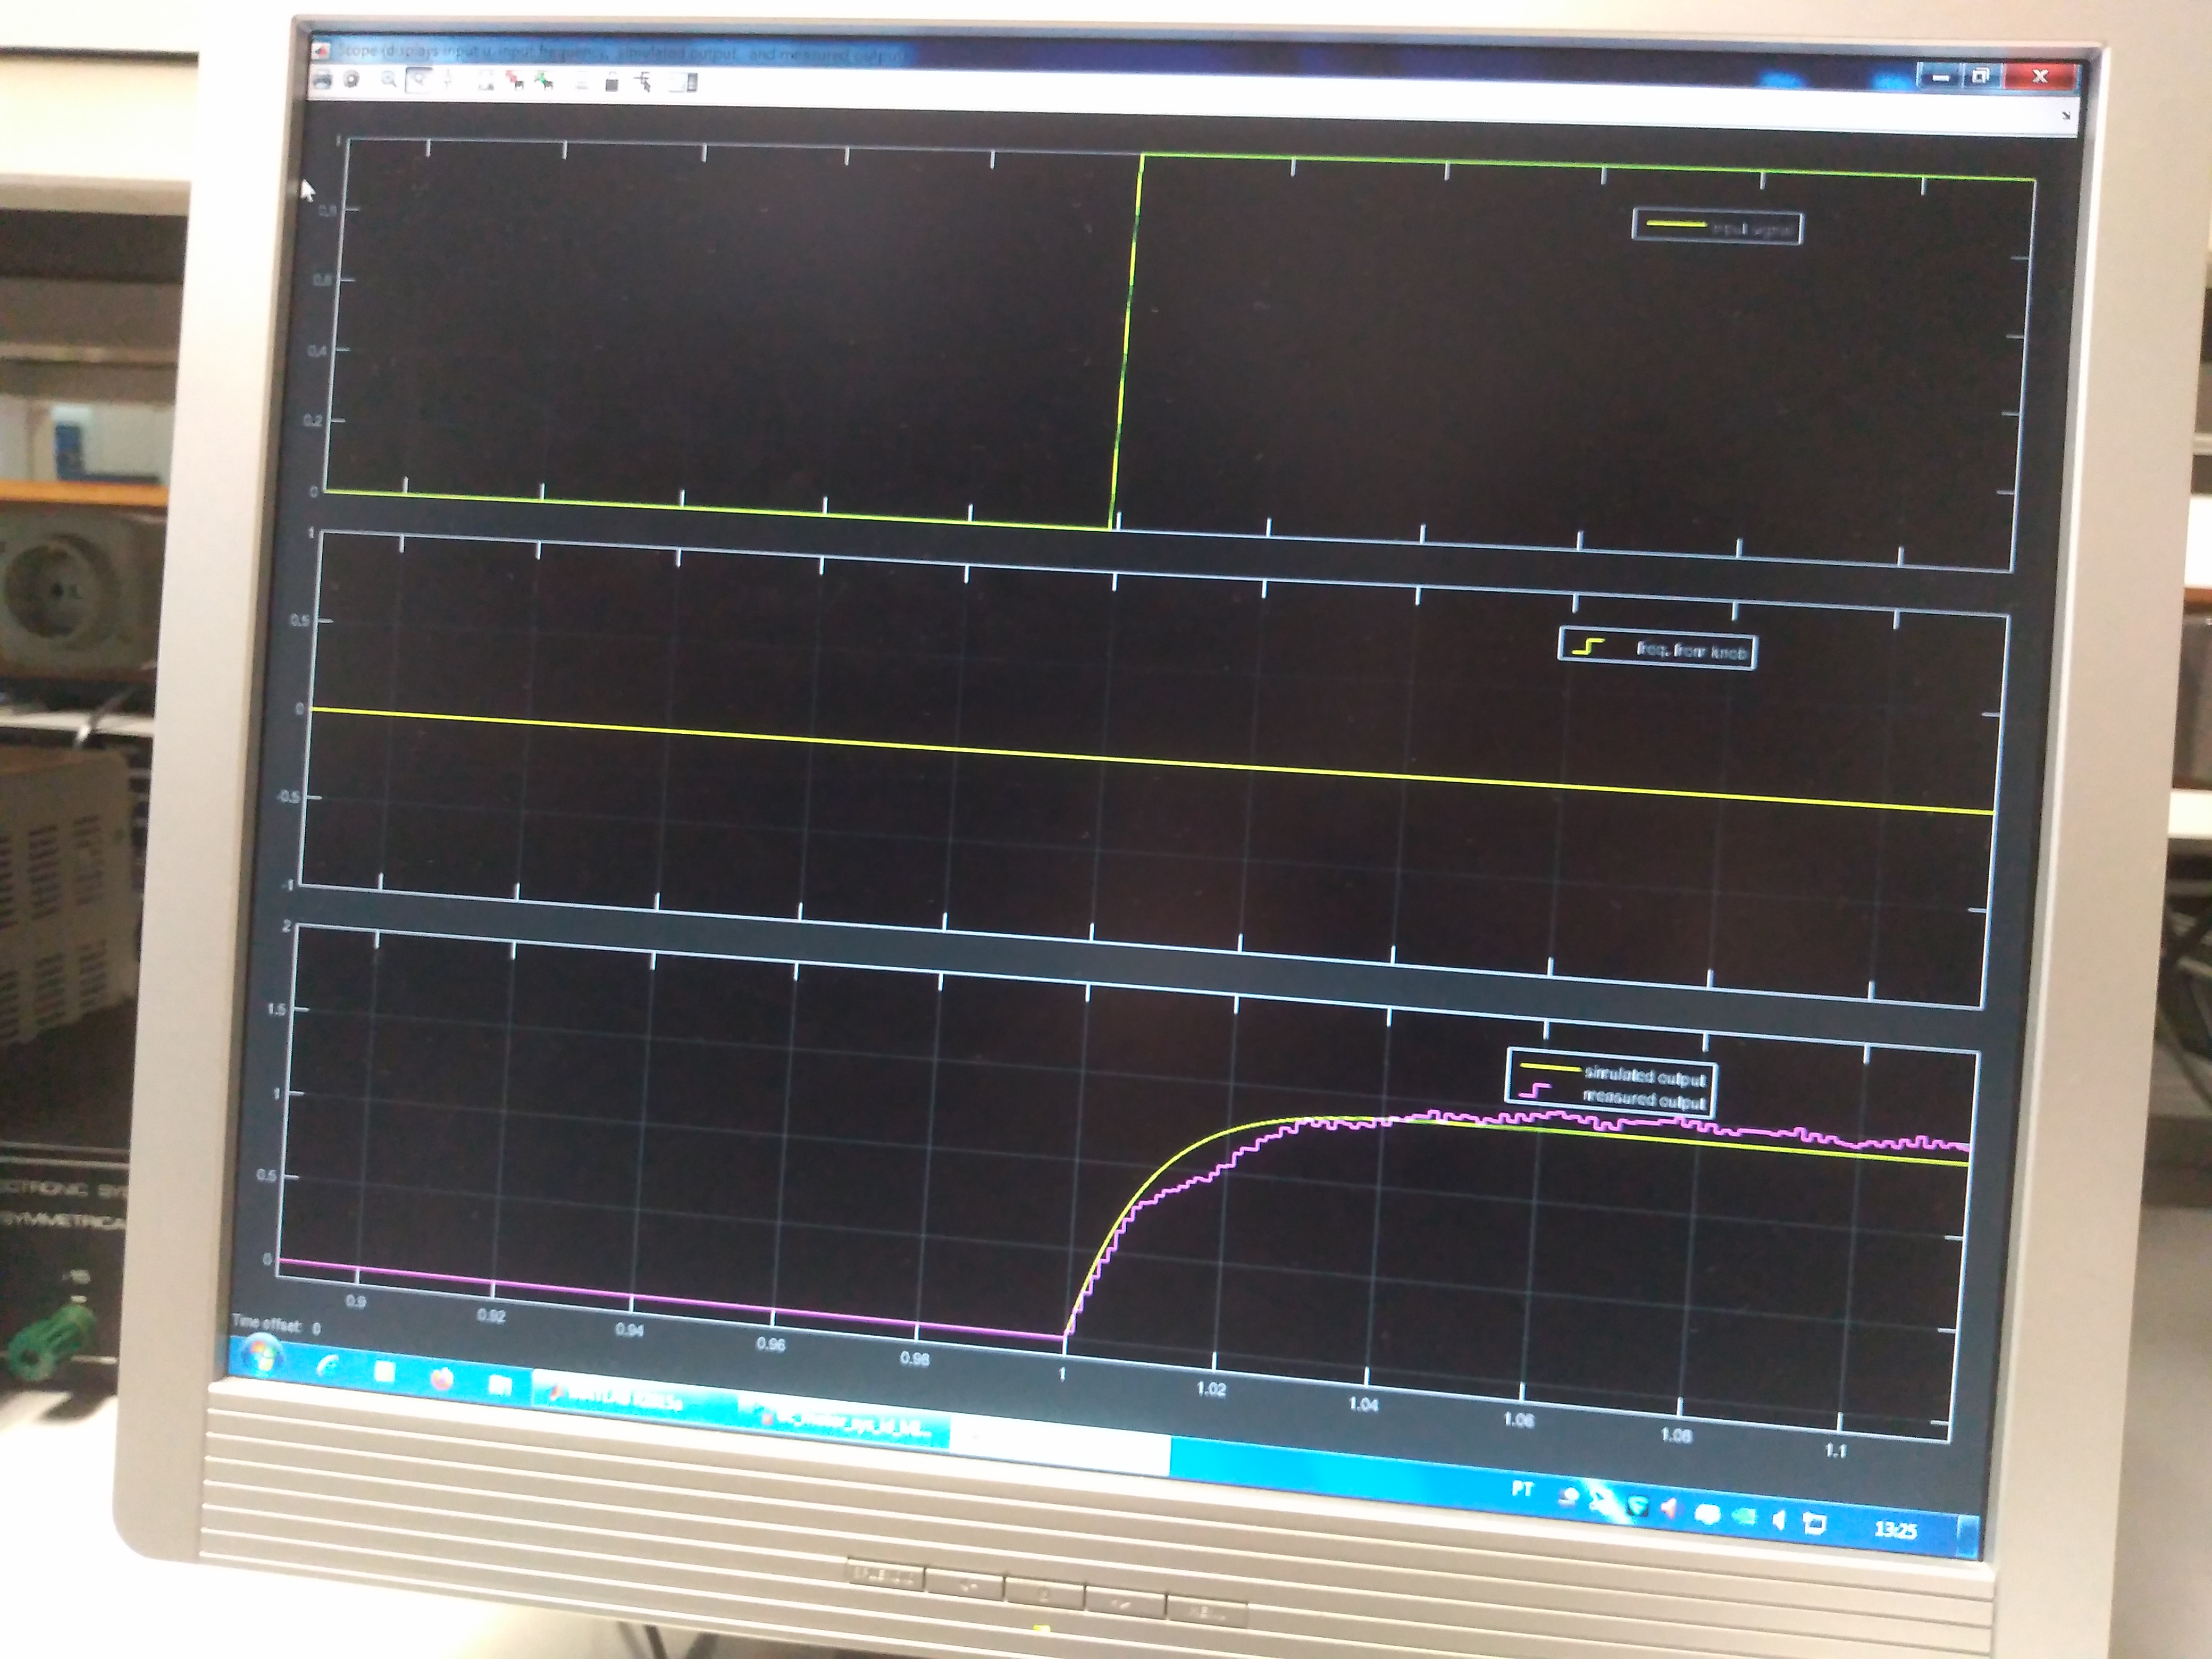
\includegraphics[width=7cm]{a107.jpg}}}%
            \qquad
            \subfloat[\centering]{{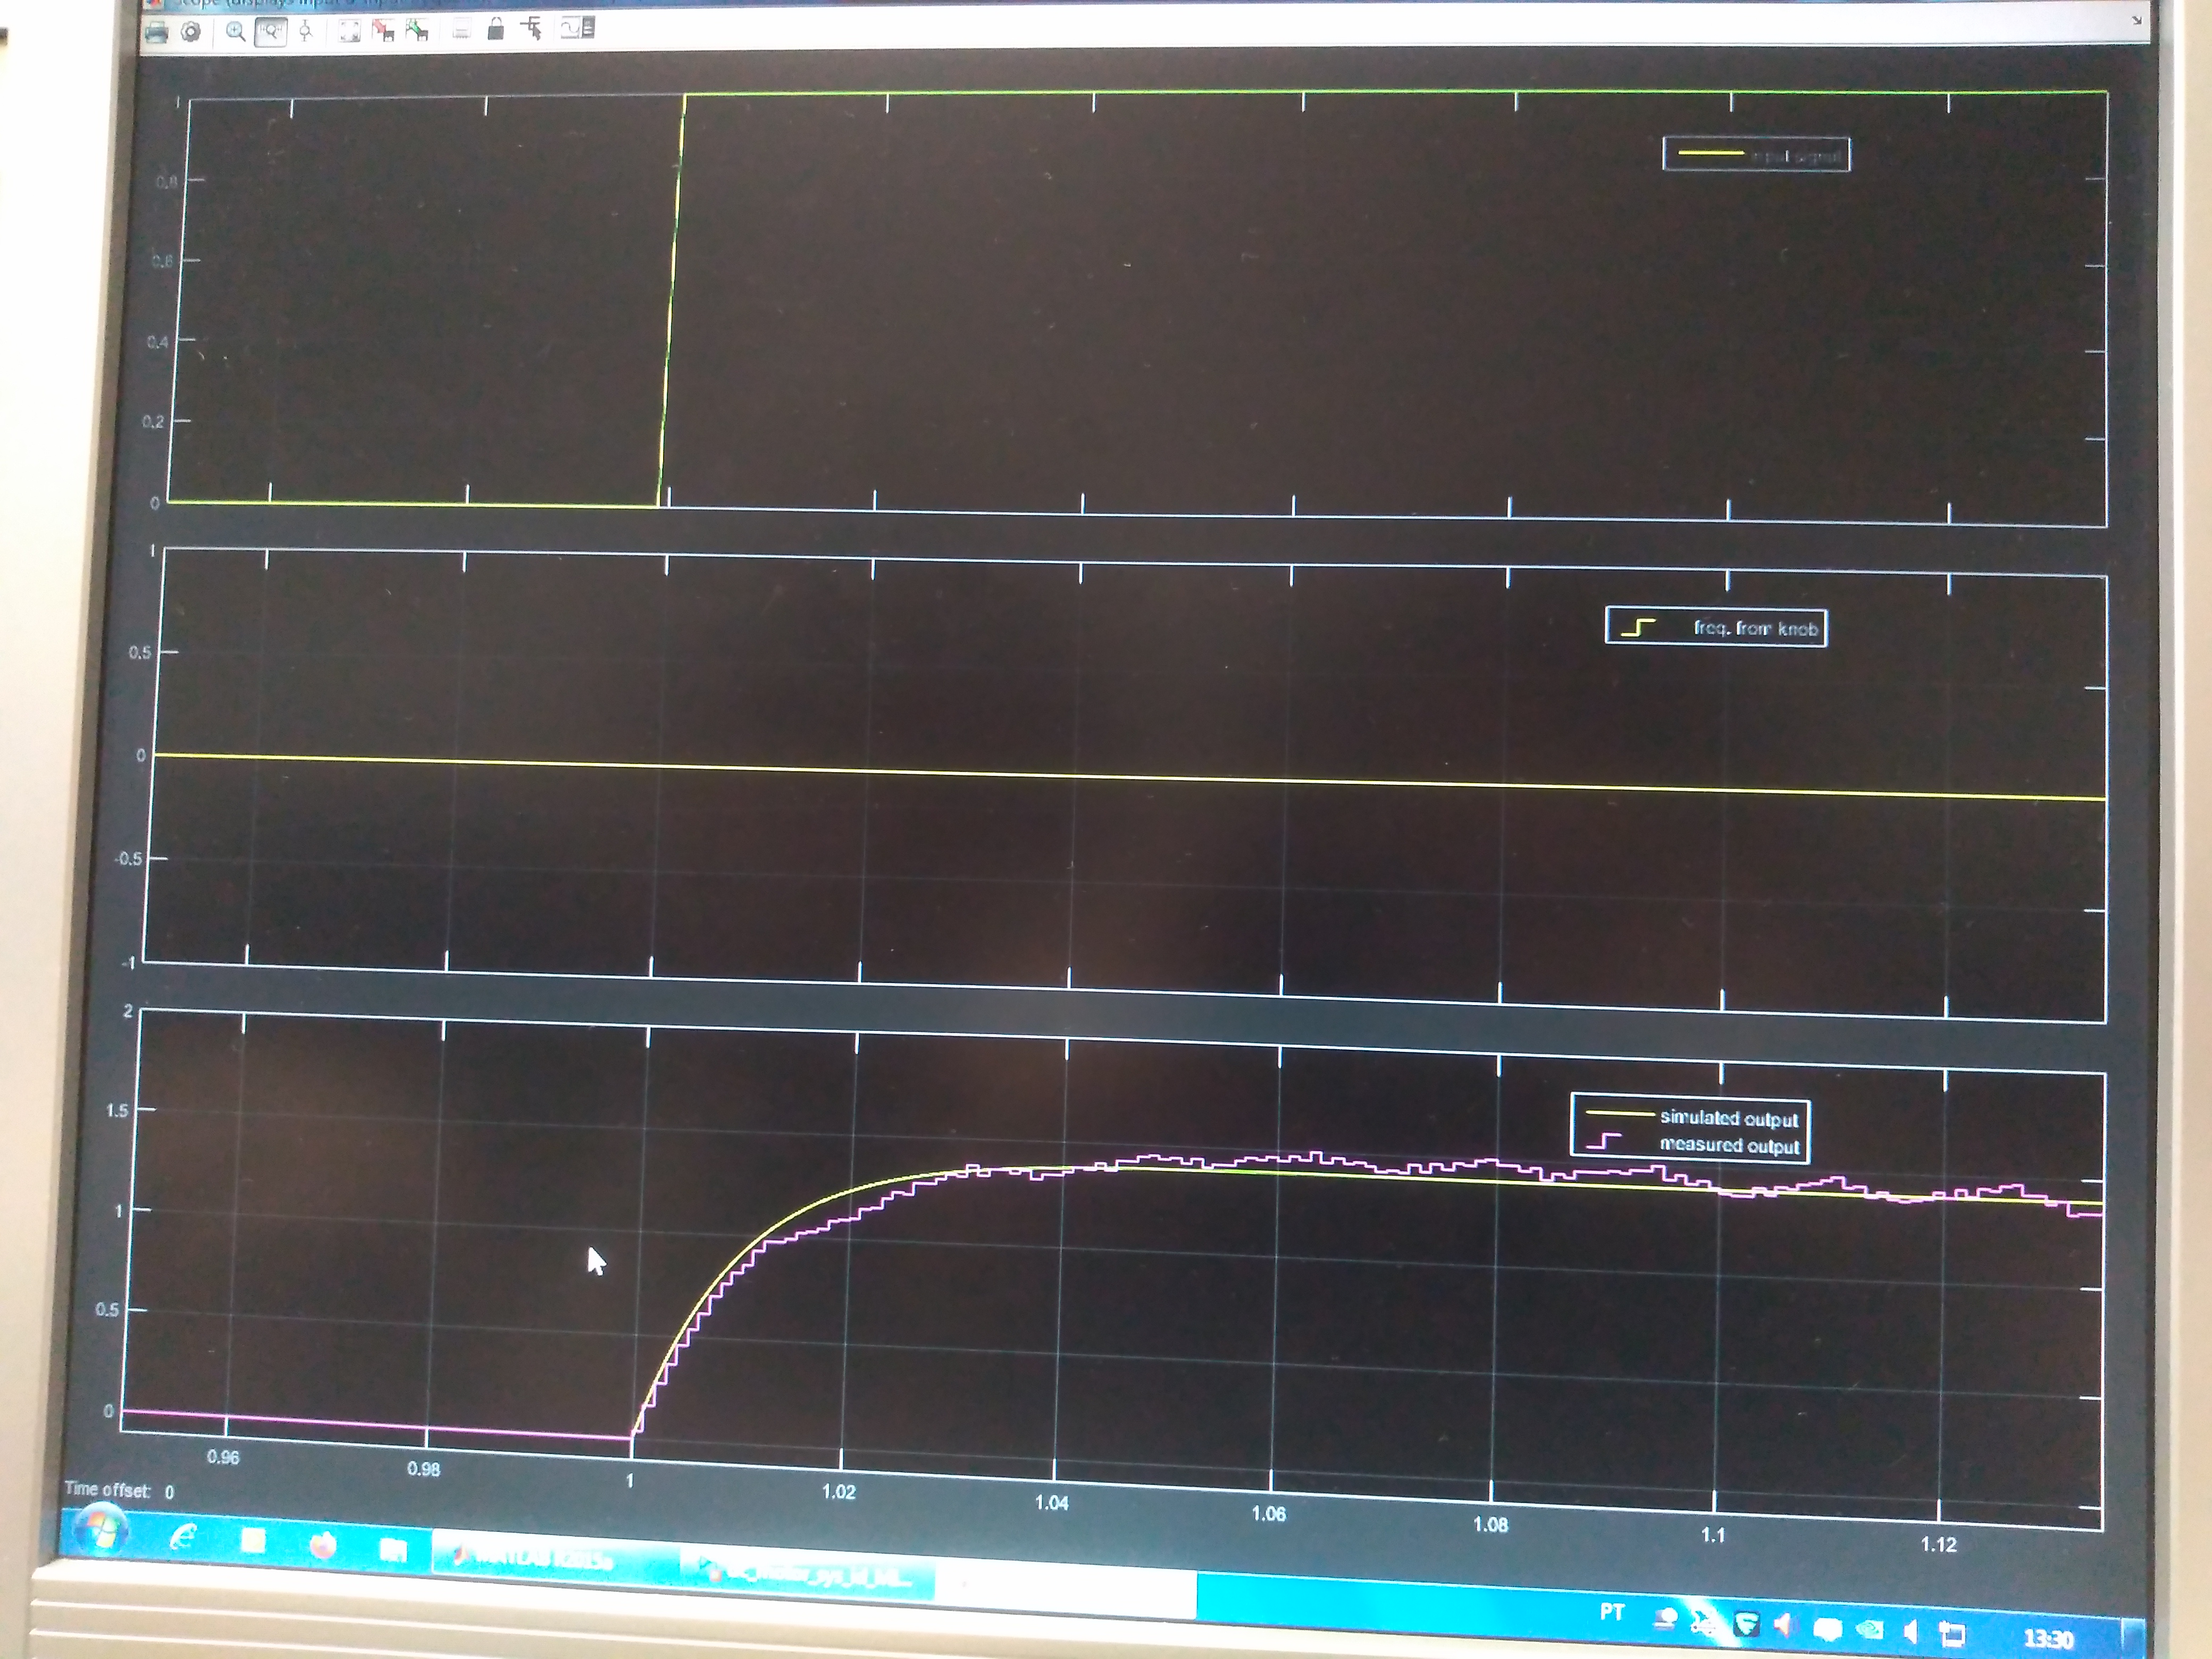
\includegraphics[width=7cm]{a_107_14.jpg}}}%
             \caption{Pictured left and right, the system response plot for both simulated (yellow) and experimental (pink) situations for $a$=107 and $a$=107.14, respectively}
        \end{figure}
        
         \clearpage
        \subsection*{Question 3.4}
        In question 3.3, we obtained a value of a=107.14. Then, we have determined values for a set of frequencies within the range [10.714; 535.7], which are in the Table 1.
       \begin{table}[H]
       \centering
        \begin{tabular}{|c||c|c|}
            \hline
            Frequency(Hz) & Amplitude(V) & gain(dB)\\ \hline\hline
            2$^1$         & 1.43         & 3.10672  \\ \hline
            5$^1$         & 1.43         & 3.10672   \\ \hline
            7$^1$         & 1.43         & 3.10672    \\ \hline
            10.714        & 0.62         & 1.87        \\ \hline
            21.428        & 0.575        & 1.21         \\ \hline
            53.57         & 0.3845       & -2.28         \\ \hline
            107.14        & 0.2285       & -6.80          \\ \hline
            214.18        & 0.102        & -13.81          \\ \hline
            535.7         & 0.0438       & -21.15           \\ \hline
        \end{tabular}
        \caption{output wave amplitude, calculated system gain and input frequency triplets}
    \end{table}
     It is important to note that the input amplitude was 0.5V.\\ 
     $^1$ In addition, we measure 3 more values at low frequencies to complete the plateau portion of the bode diagram, it is important to note that these values were take for an input amplitude of 1V . 
    
    \subsection*{Question 3.5}
        From question 3.3, we estimated the value of $a$ = 107.14 and $K_0$=1.4. Substituting these values in the transfer function, and using MATLAB, it is possible to compute the theoretical Bode diagram.   
        With the values obtained in the previous question we can compute a Bode plot of the gain-frequency relation function: 
           \begin{figure}[ht]
            \centering
            \captionsetup{justification=centering}
            \subfloat[\centering]{{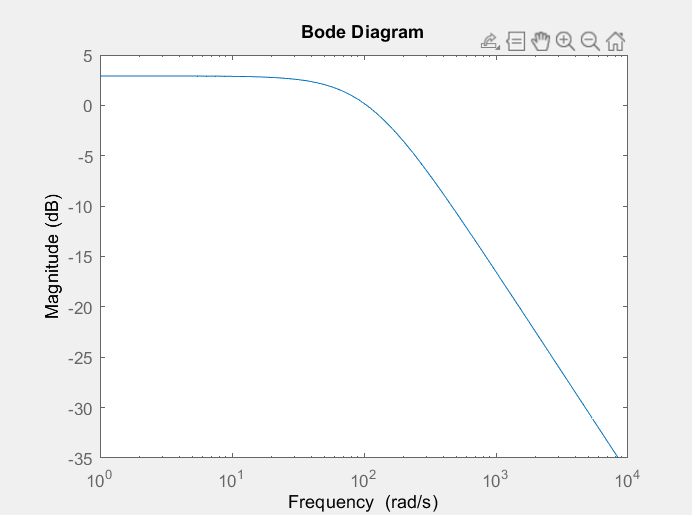
\includegraphics[width=0.45\textwidth]{3_5_New.png}}}%
            \qquad
            \subfloat[\centering]{{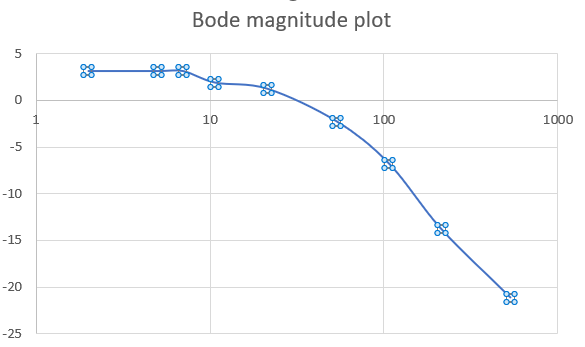
\includegraphics[width=0.45\textwidth]{3_5V2.png}}}%
        \caption{Pictured left and right, the theoretical Bode plot of the function G(s) and the experimental Bode magnitude plot, respectively}
        \end{figure}
        \\ It is important to note the "plateau" discrepancy between the values obtained at 1V (predicted "plateau" at 3.1 dB) and 0.5V, which leads us to conclude that the motor had a faulty operation for the input voltage interval of [0.5, 1[ V, which could also explain why the experimental cutoff frequency is visibly inferior to 107.14 Hz, as it was predicted.
        \clearpage
        \subsection*{Question 4.4}
        With the values computed in question 4.1, we found that for negative values of the real zero, the motor had an erratic behaviour, effectively adding a similar to time-delay component and a persistent overshoot to the system.\\
        \begin{figure}[ht]
            \centering
             \captionsetup{justification=centering,margin=2cm}
            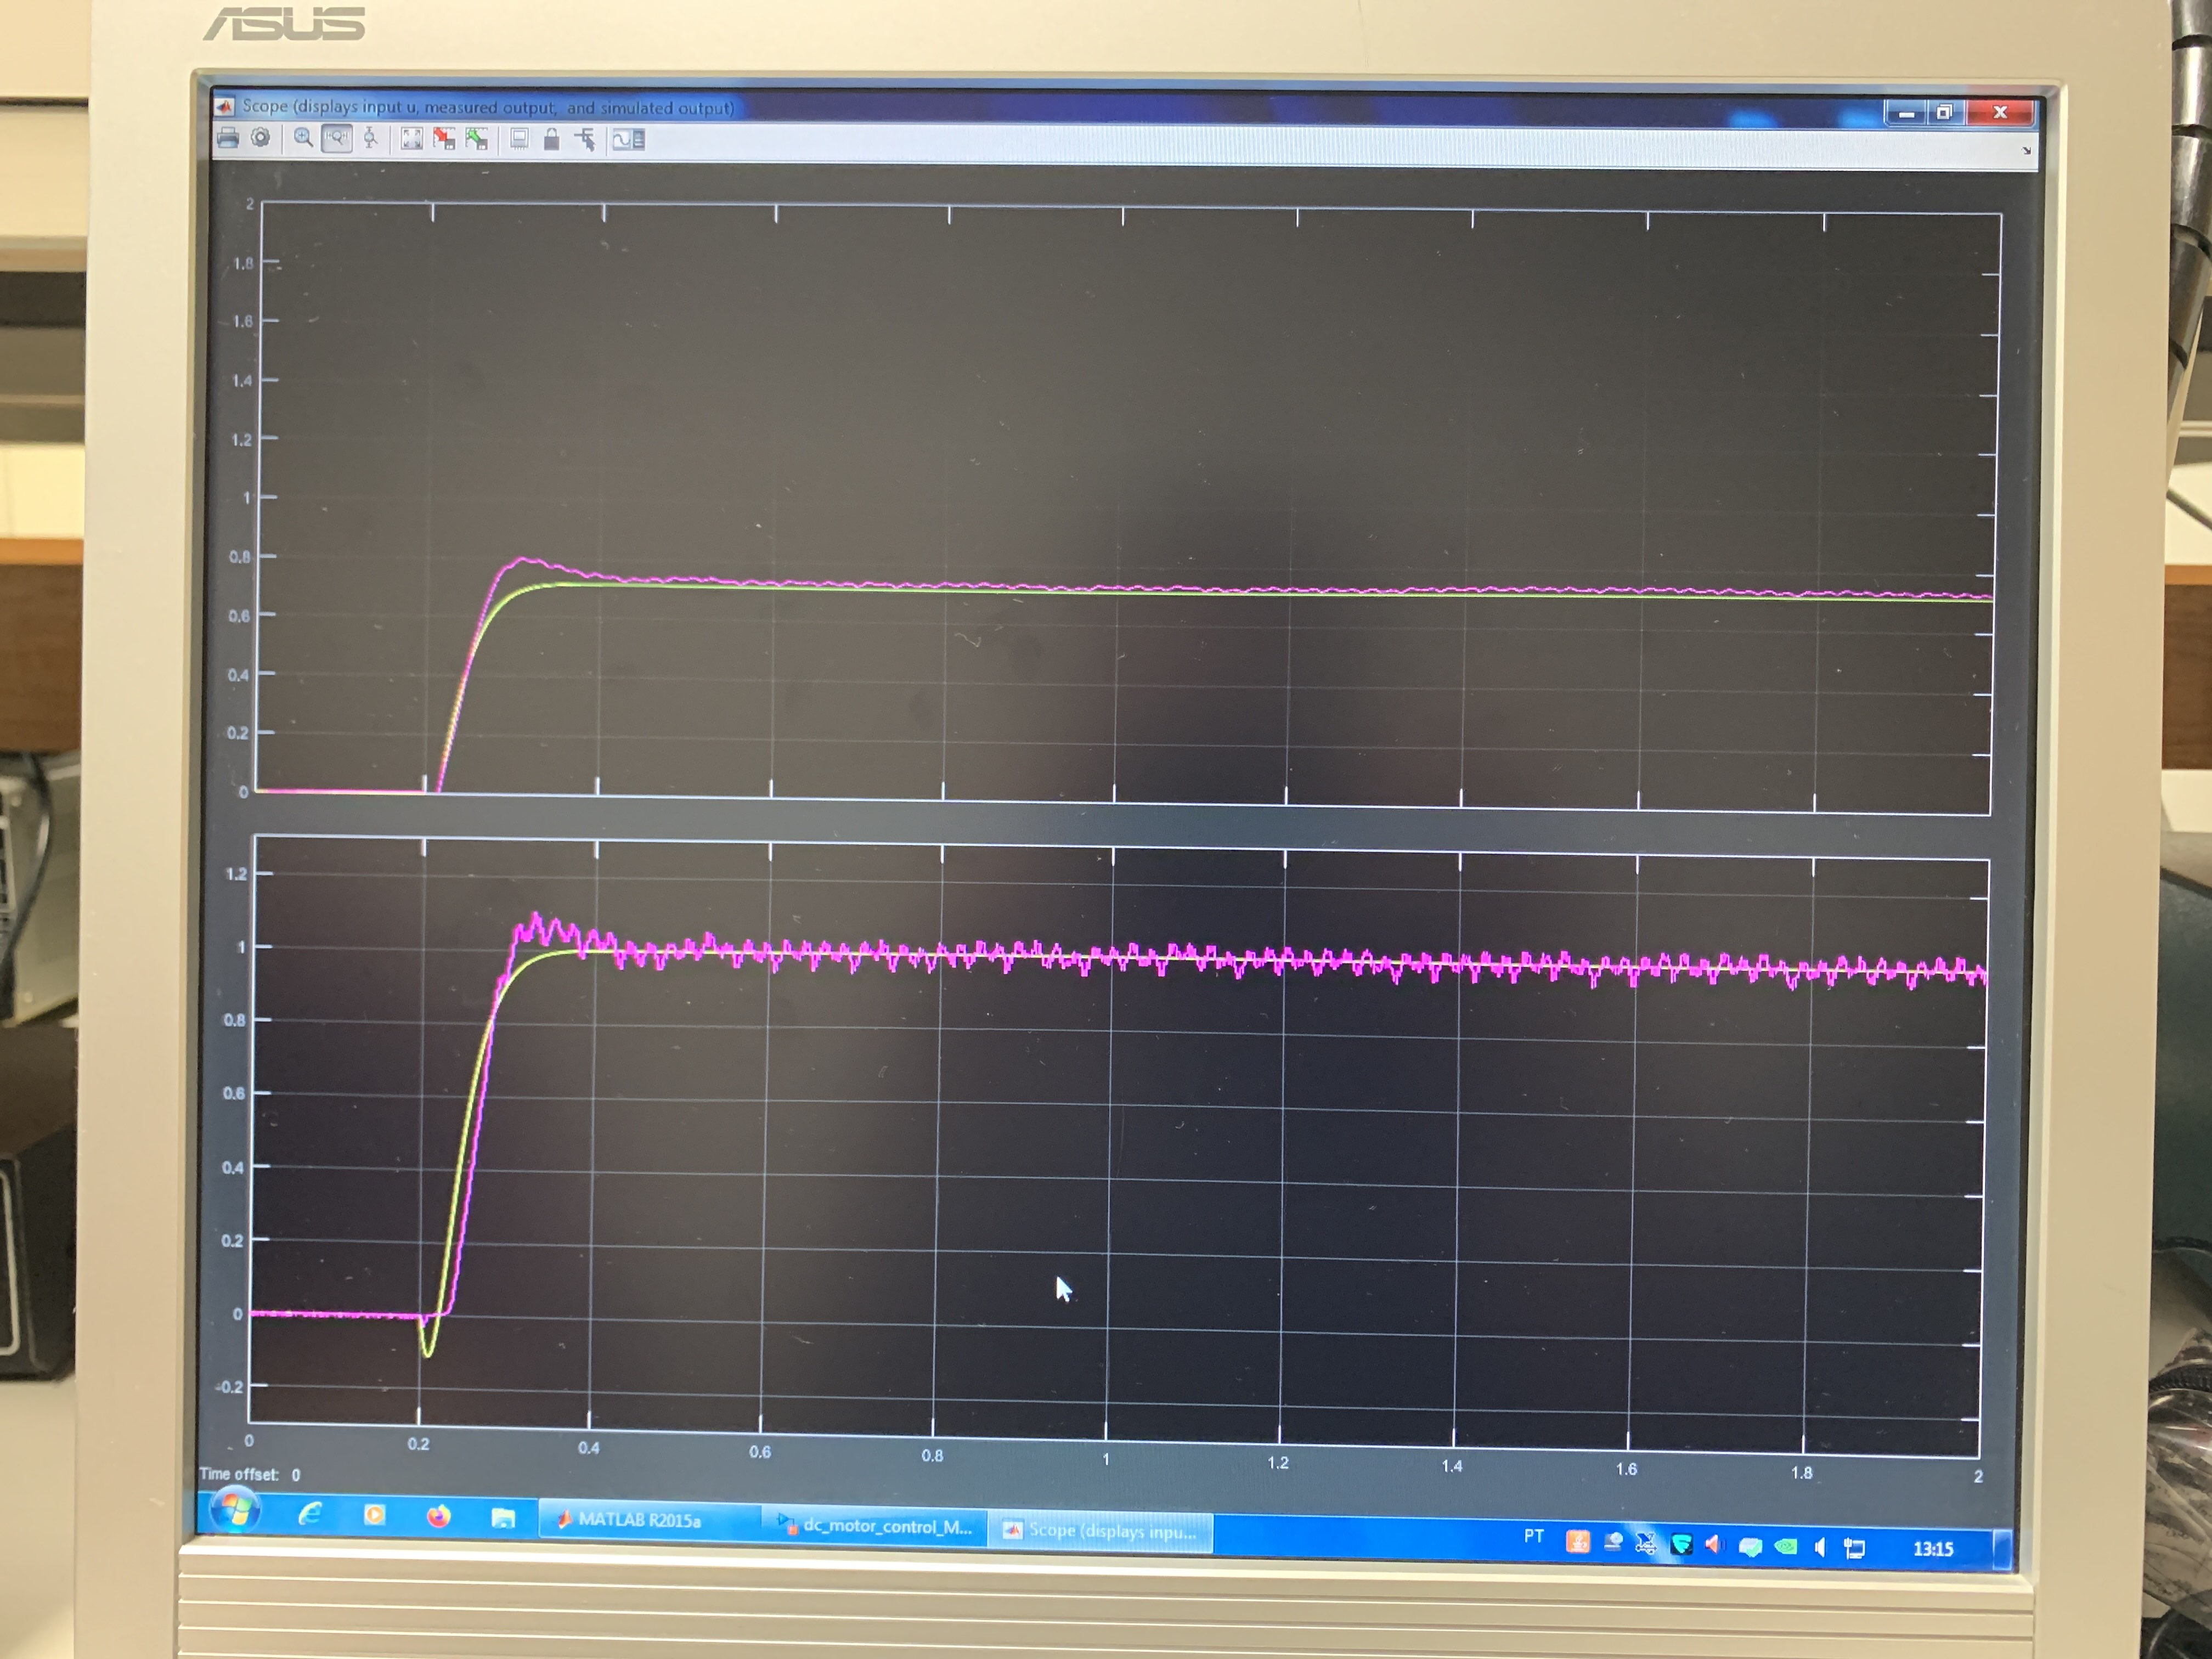
\includegraphics[width=9cm,height=5cm]{negativezero.jpg} 
            \caption{Step response of the simulated system with $k_1$ = 12 and $z$ =-67.}
        \end{figure}
        After observing such results and after reviewing the laboratory guide we made the zero positive, this is, $z$ = 67. Doing so, the motor behaved as predicted, and the actual step response was much more similar to the simulated one.
        \\ An even better response was obtained when we adjusted $k_{1}$ to 11, as shown below:
            \begin{figure}[ht]
            \centering
             \captionsetup{justification=centering,margin=2cm}
            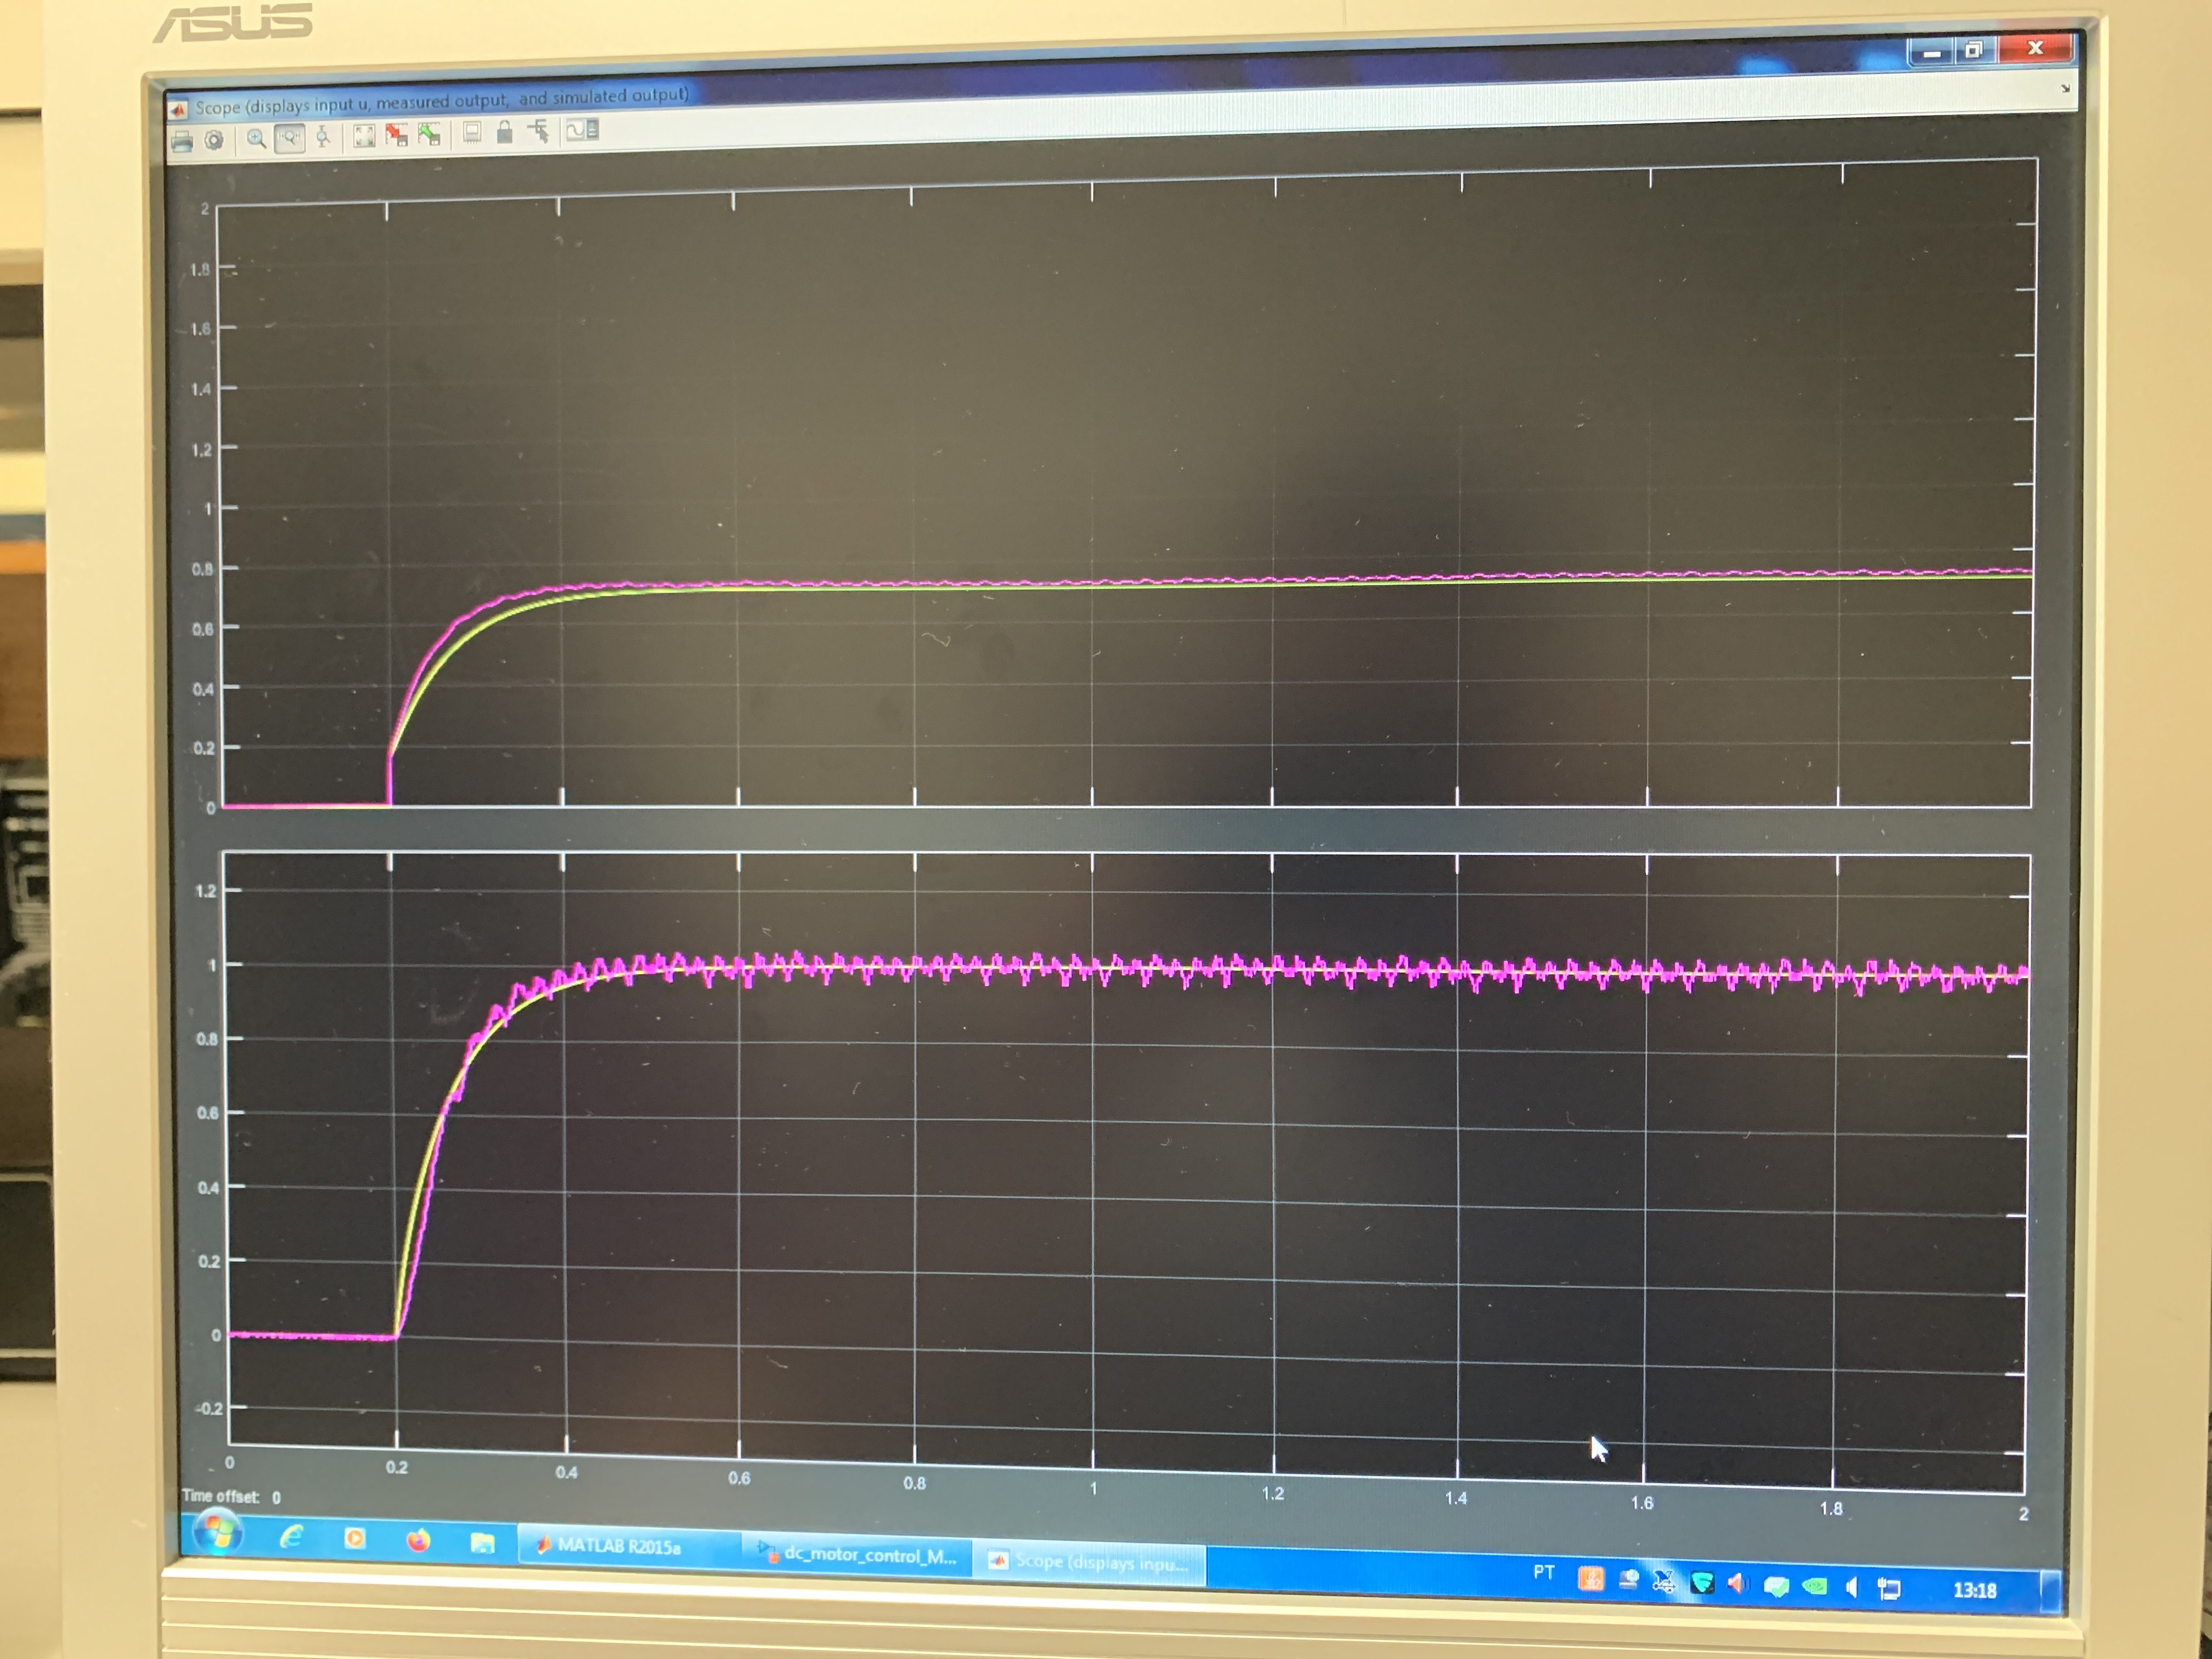
\includegraphics[width=9cm,height=5cm]{4_4.jpg} 
            \caption{Step response of the simulated system with $k_1$ = 11 and $z$ = 67.}
        \end{figure}
        \clearpage
        \subsection*{Question 4.5}
        In order to observe evidences of overshoot, we had to push the system static gain, which was achieved through assigning $k_1$=200 and following up with $z$=120
          \begin{figure}[ht]
            \centering
             \captionsetup{justification=centering,margin=2cm}            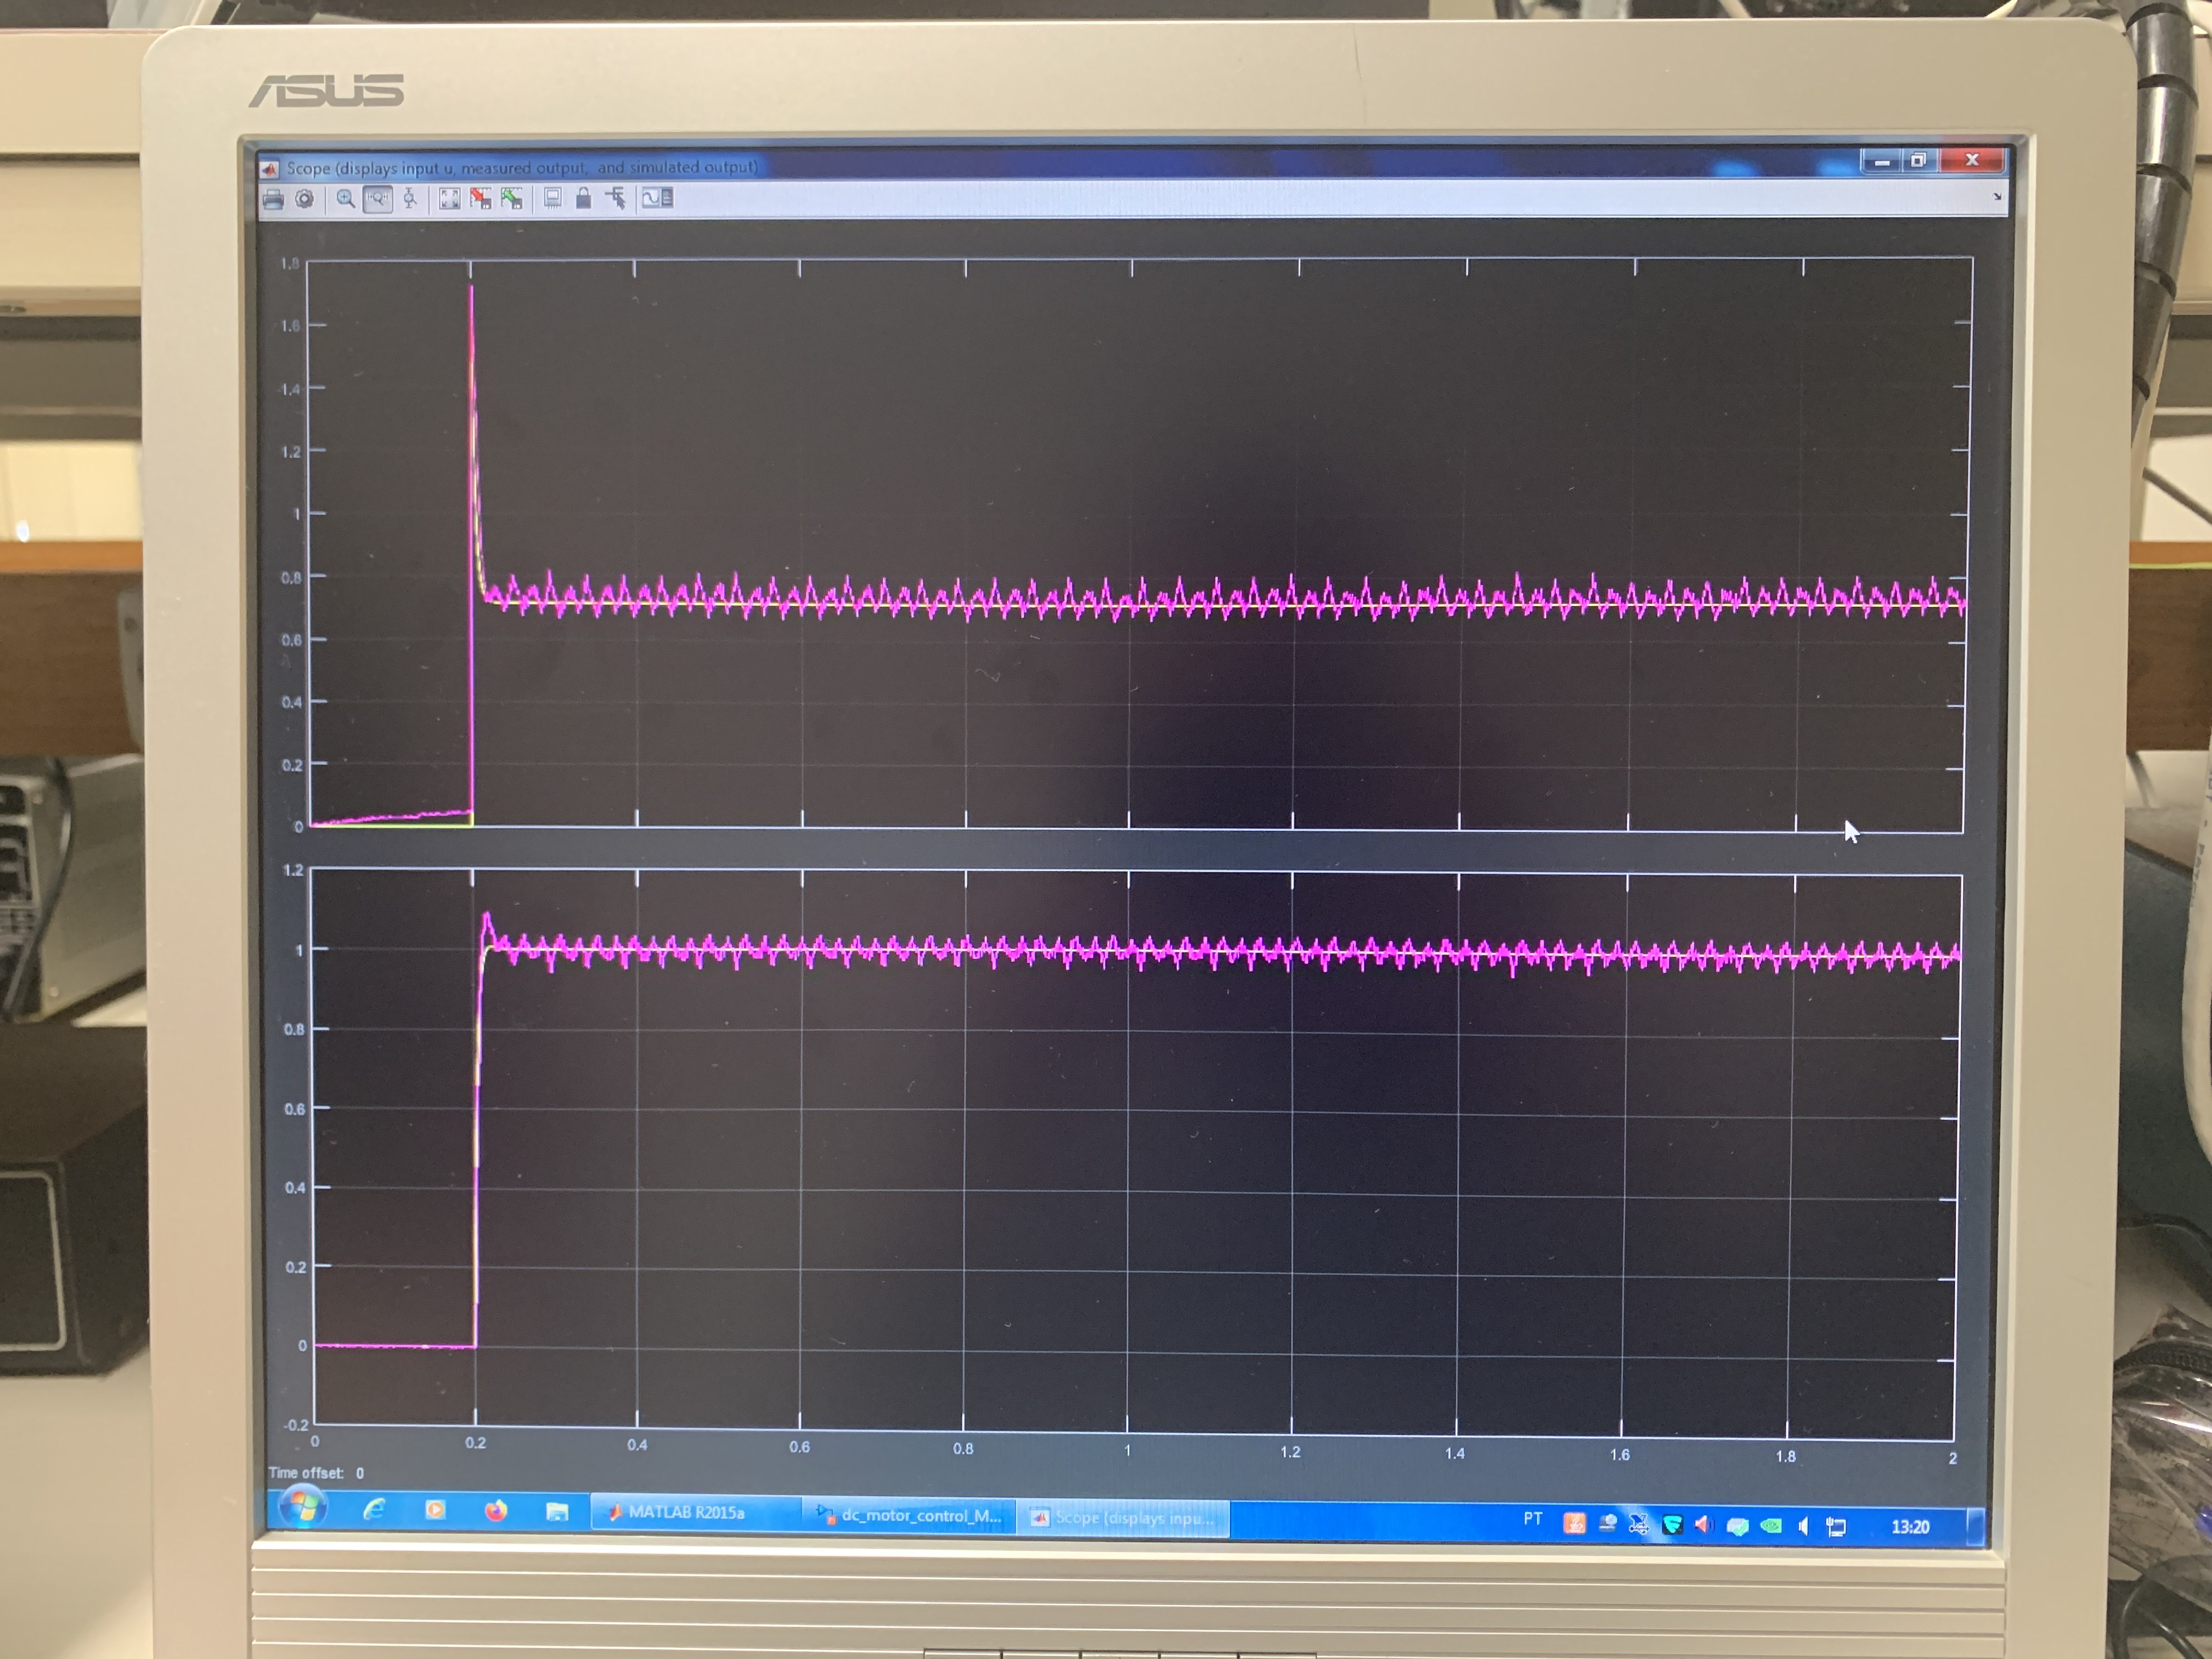
\includegraphics[width=9cm,height=5cm]{4_5.jpg} 
            \caption{Step response of the simulated system with different values of $k_1$ and $z$.}
        \end{figure}
    
        \begin{figure}[H]
            \centering
             \captionsetup{justification=centering,margin=2cm}
            \subfloat[\centering]{{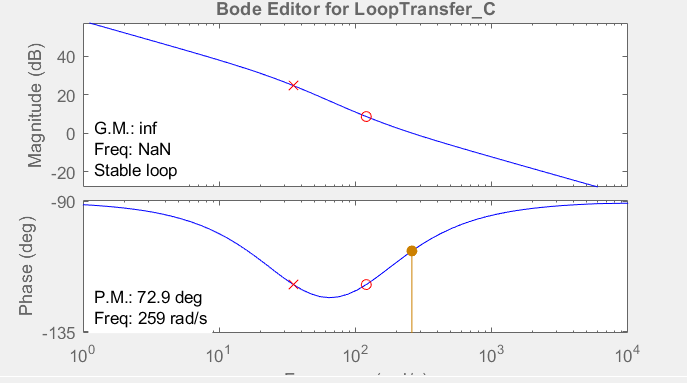
\includegraphics[width=0.45\textwidth]{pmk200.png}}}%
            \subfloat[\centering]{{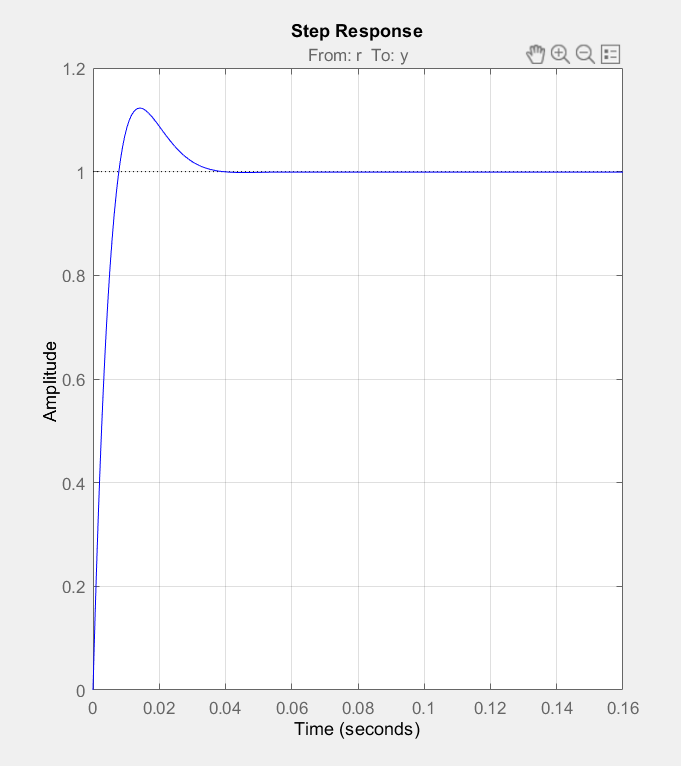
\includegraphics[width=0.3\textwidth]{srk200.png}}}%
            \caption{Phase Margin(a) and time response(b) simulation diagrams for $k_1$=200 and $z$=120}
        \end{figure}
        \begin{figure}[H]
            \centering
             \captionsetup{justification=centering,margin=2cm}
            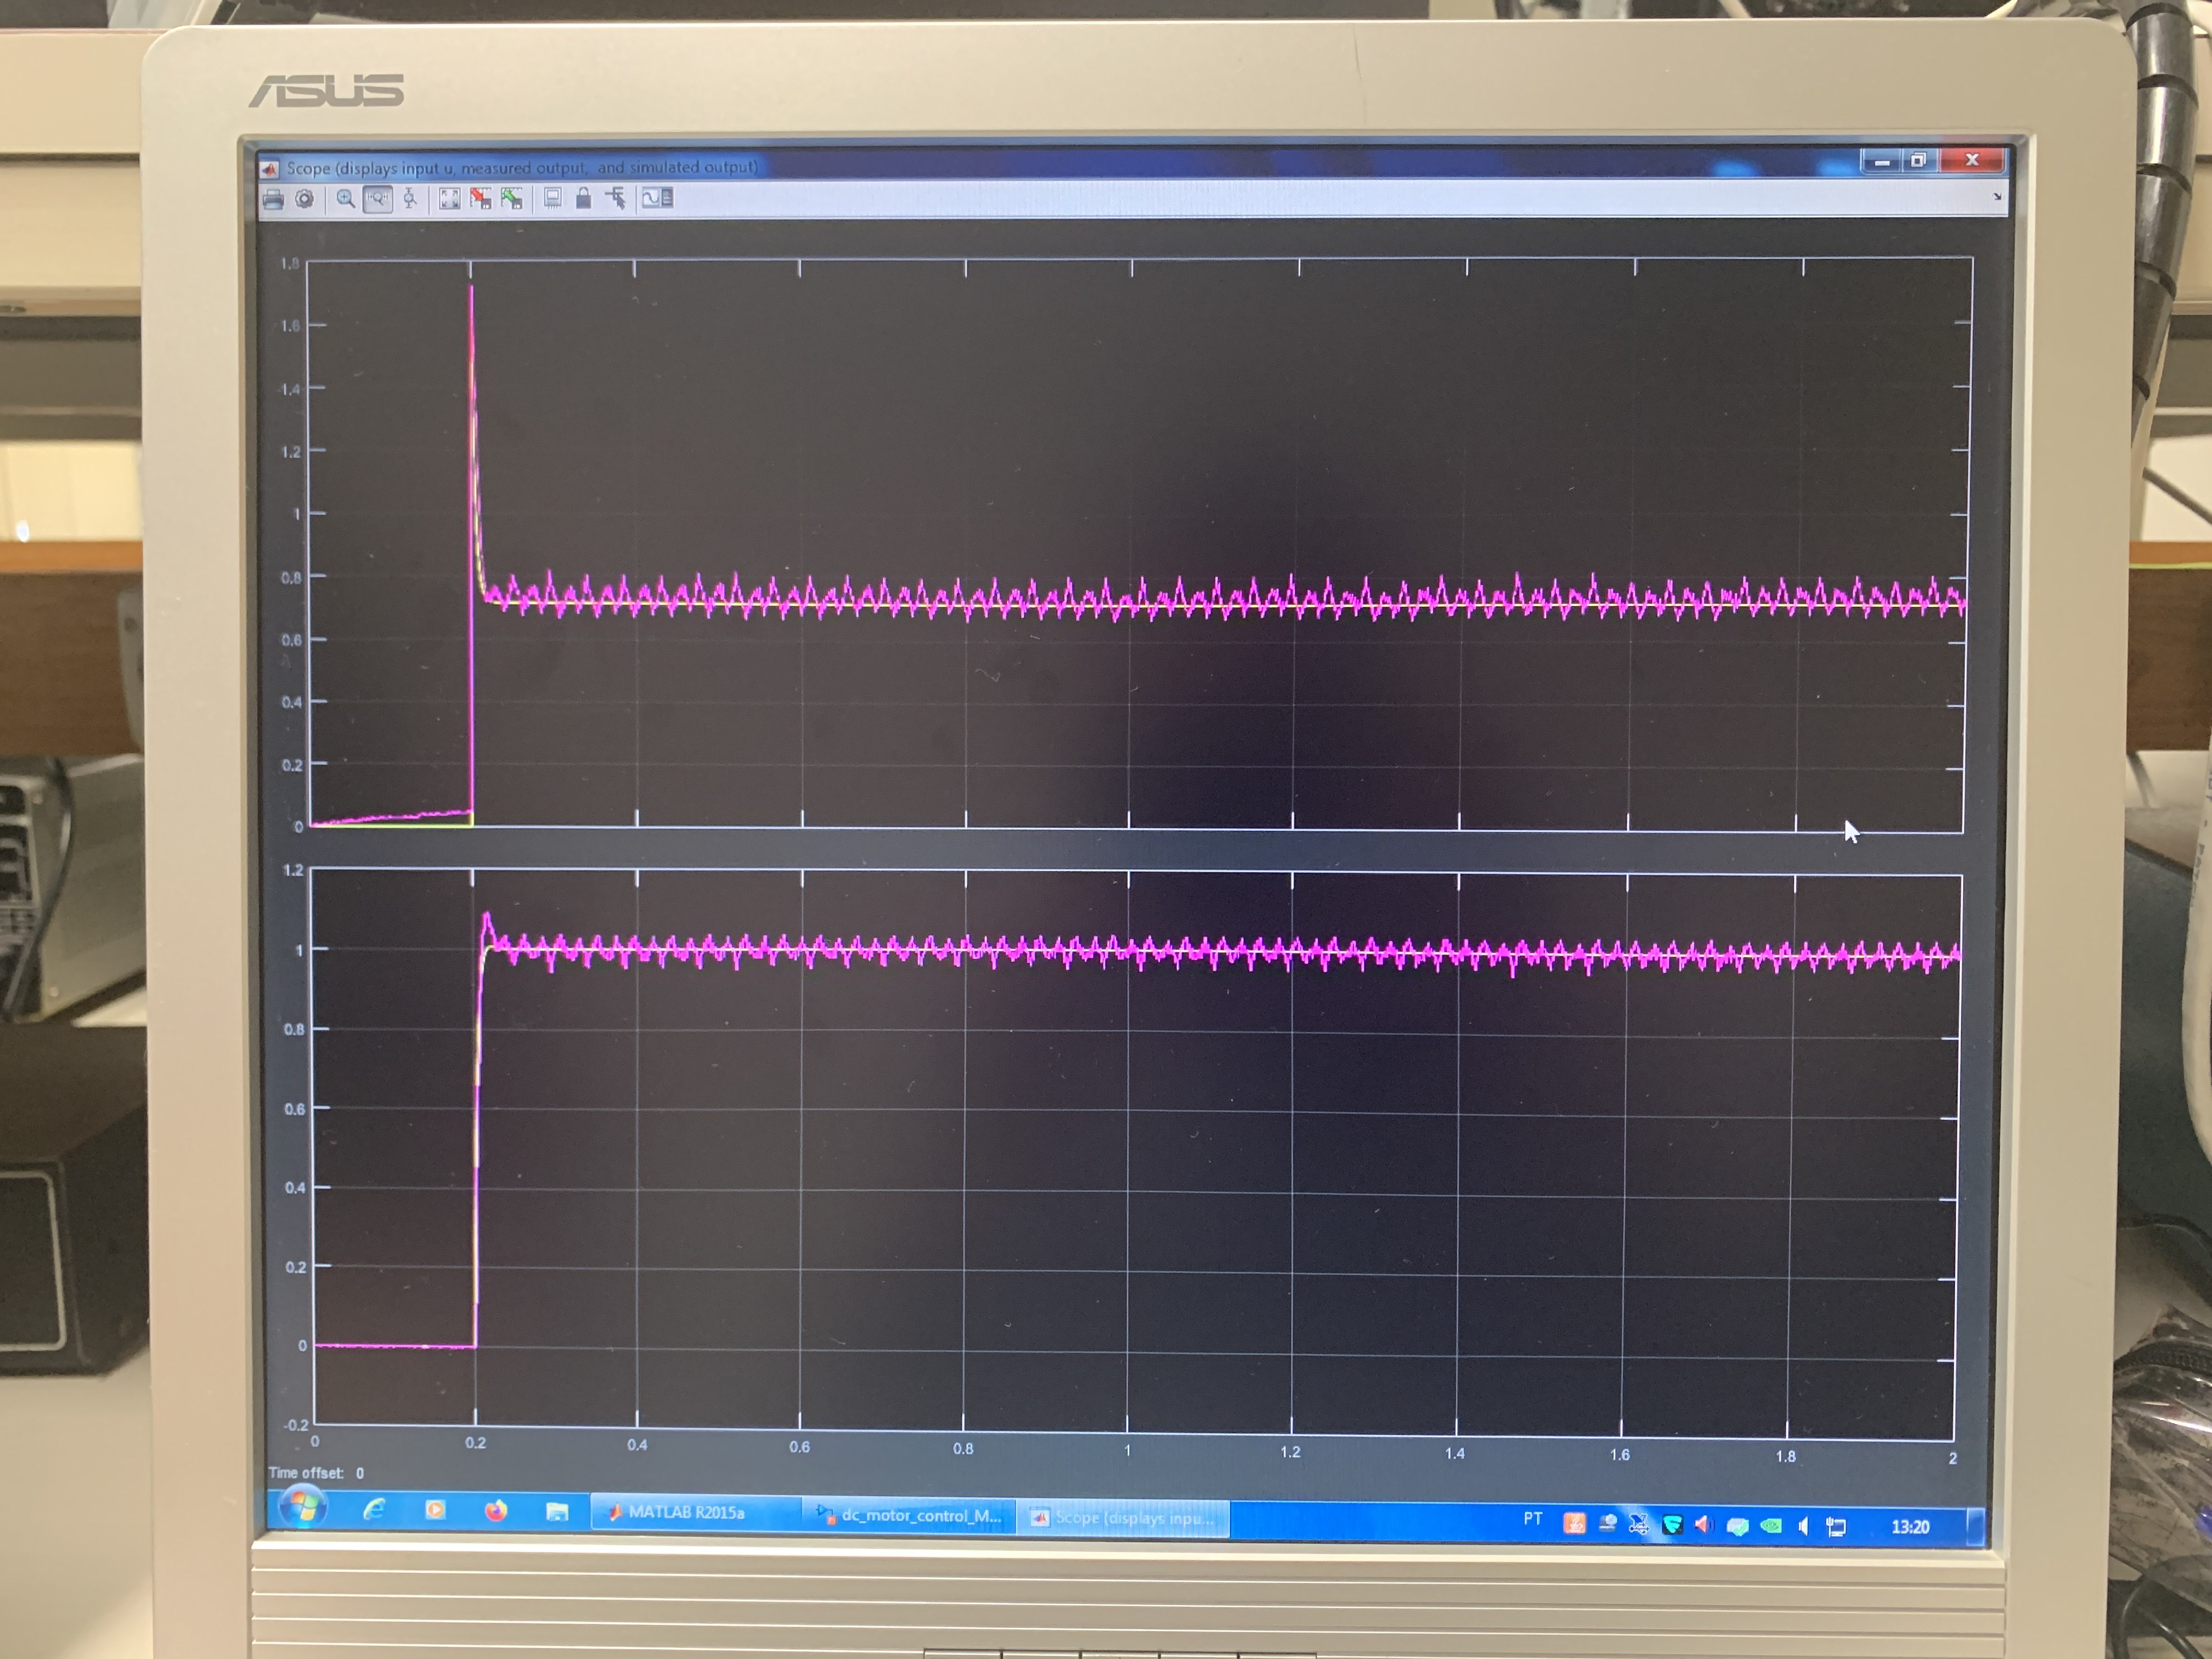
\includegraphics[width=9cm,height=5cm]{4_5.jpg}
            \caption{System root locus diagram for $k_1$=200 and $z$=120. Note the two closed loop imaginary poles which explain the observed under-damped response}
        \end{figure}
        
         We can see that by increasing $k_1$ and making the zero closer to the pole, the peak overshoot value skyrockets, inferring an almost marginal stability. Additionally we can verify that the phase margin minimum is the overshoot maximum.
         Finally we can also verify,through gain modification, that the crossover frequency and peak time are inversely proportional.
        \subsection*{Question 4.6}
        In this question, we want to observe the effect of the time delay on the performance of the system. For that, we changed the switch of the MATLAB's ControlSystemDesigner in order to add the time delay. The result obtained is in the figure 12 and, with the different parameters $k_1$ and $z$ .
        \begin{figure}[ht]
            \centering
            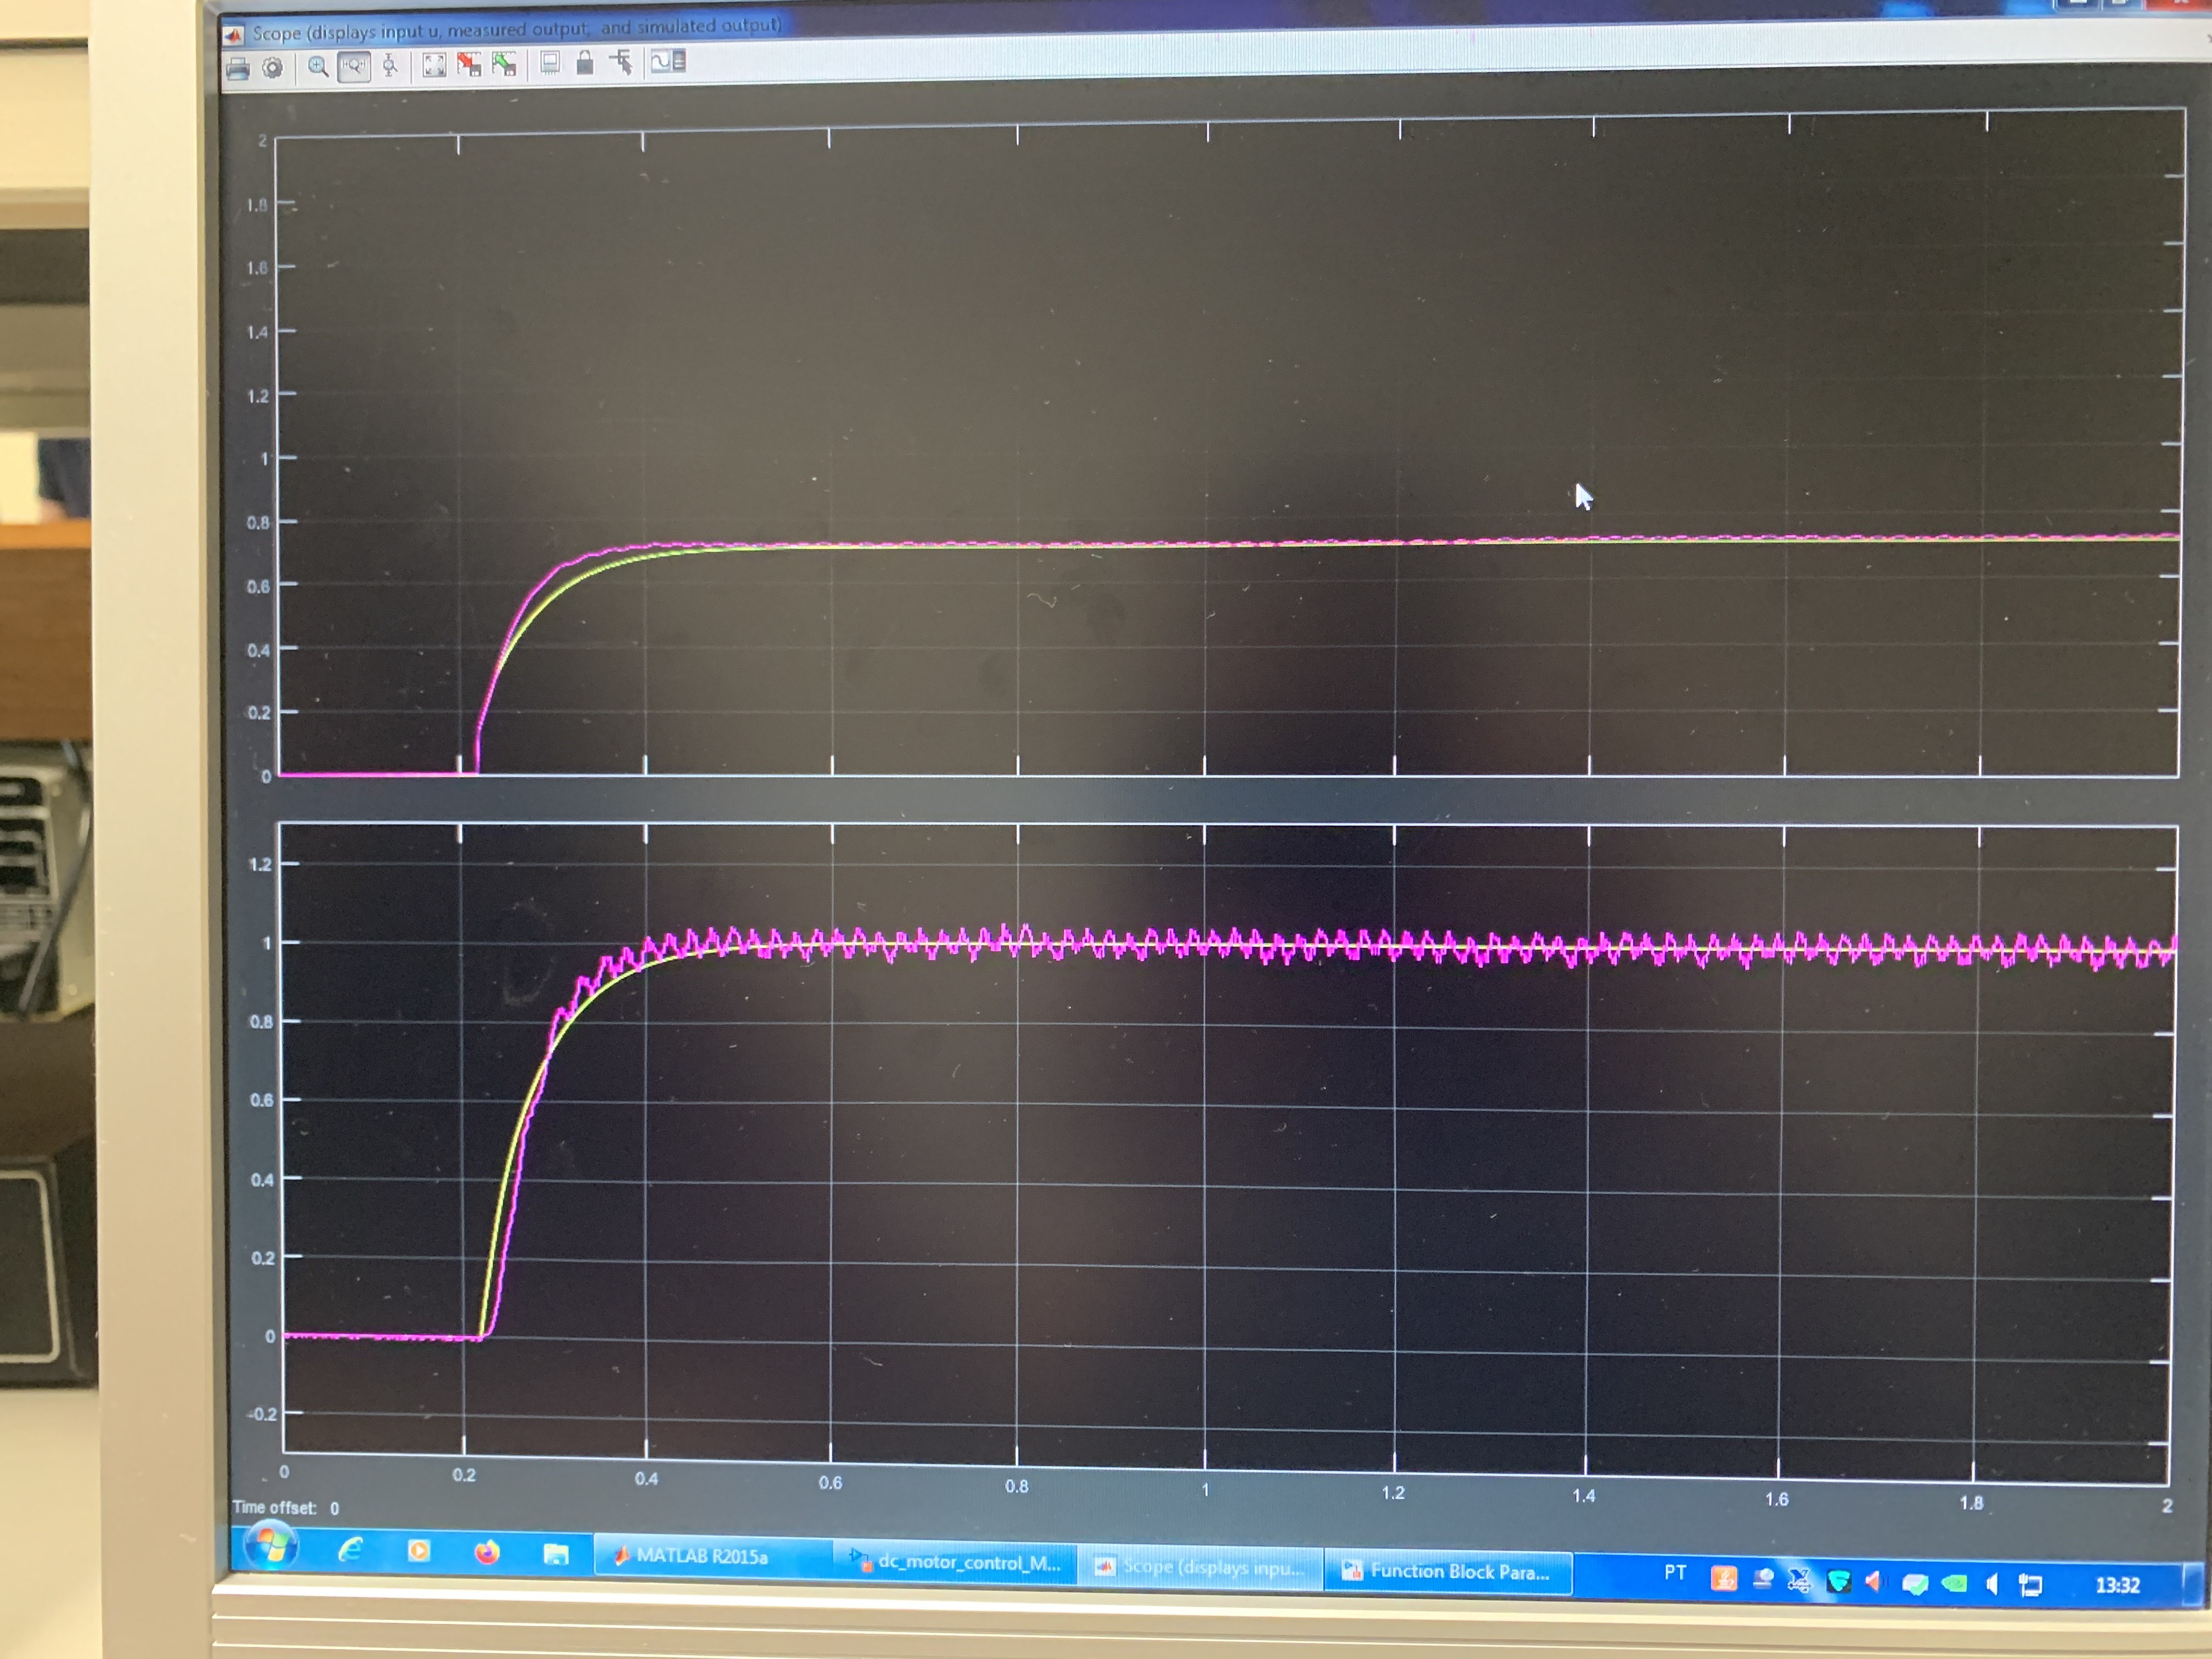
\includegraphics[width=9cm,height=5cm]{4_6new.jpg} 
            \caption{Step response of the simulated system with time delay, and values of $k_1$ = 9 and $z$ = 67.}
        \end{figure}
        
          \begin{figure}[ht]
            \centering
            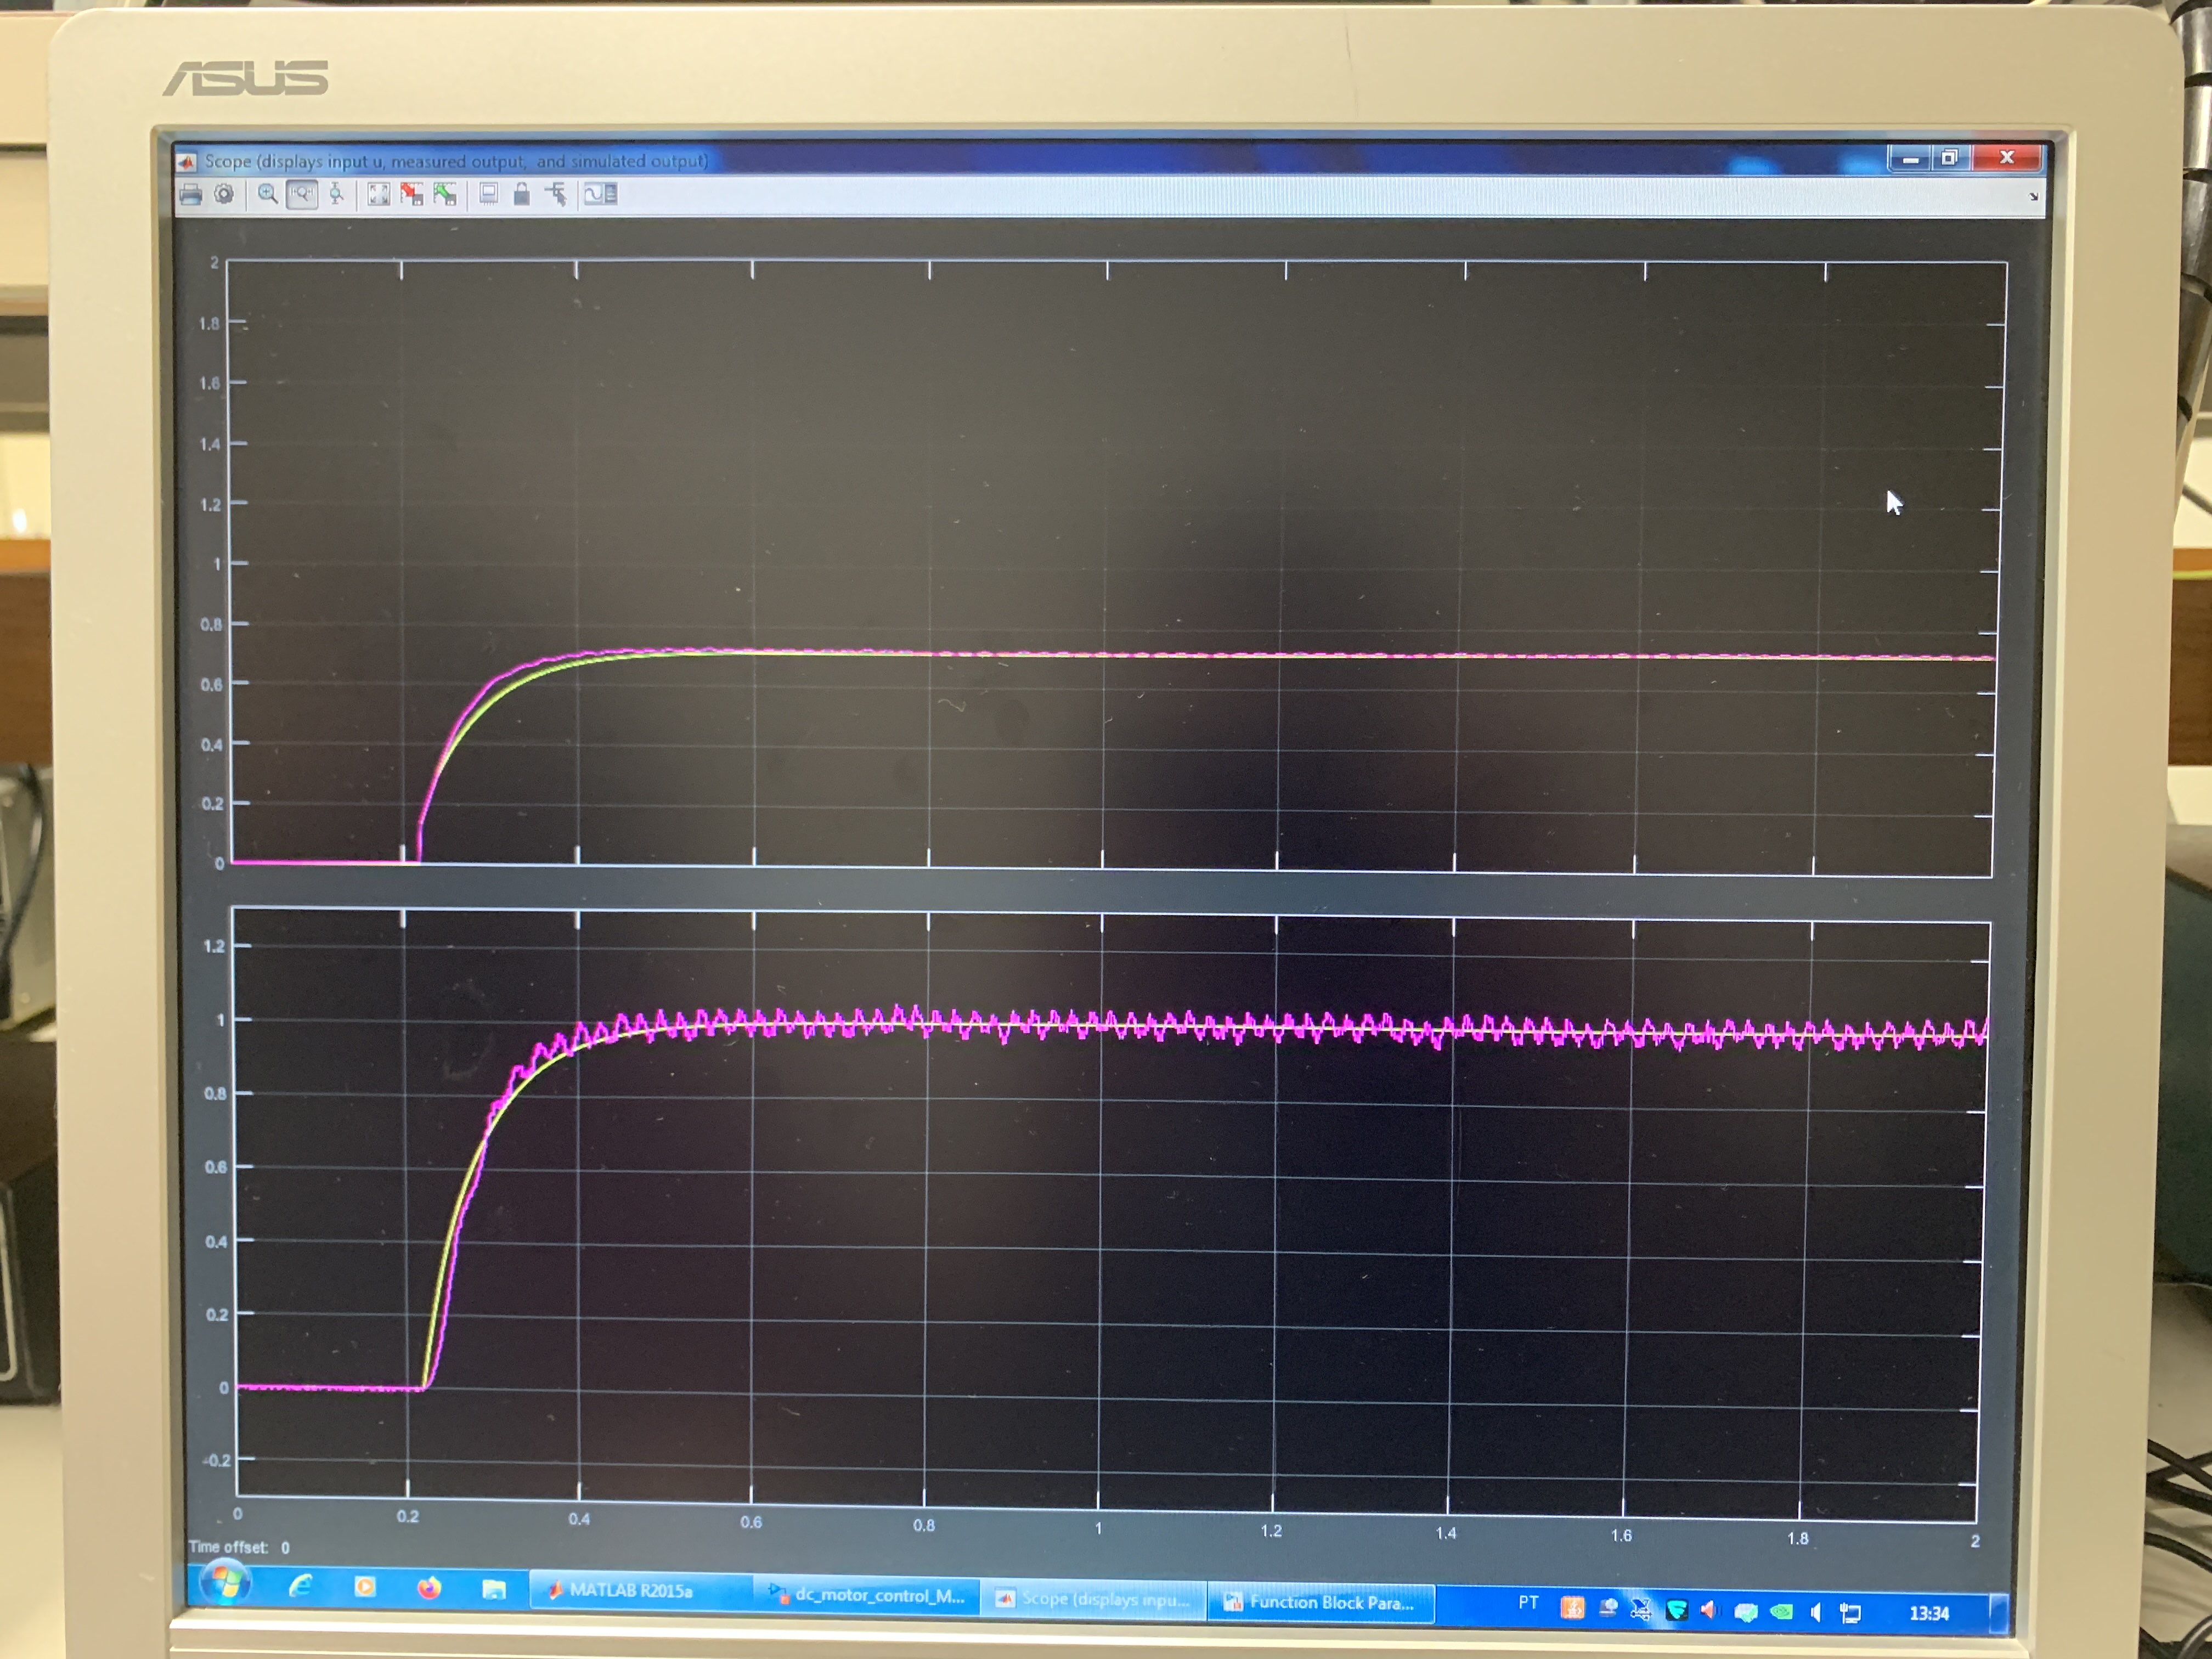
\includegraphics[width=9cm,height=5cm]{4_6_2.jpg} 
            \caption{Step response of the simulated system with time delay, and values of $k_1$ = 8.5 and $z$ = 66.7.}
        \end{figure}
        \section{Conclusions}
        This laboratory sessions allowed us to learn how to apply automatic Control theory onto an actual, real physical system.\\
        
        We learned how to use theoretical tools such as the root locus and Nyquist diagrams, which gave us some prediction power in the system context, which in turn helped us project the PI controller used in order to dictate the motor's behaviour.\\
        
        We soon understood that between a simulation and real-life there is a big behavioural rift that is, however, predictable, as the real world is far from ideal, with systematic noise, operational intervals and occasional random events that affect the observations.\\
        
        Still, we can state that our experiments were quite satisfactory, and that if we faced the motor as a experimental black box, with no previous simulation and predictive knowledge, the following assignment would have taken a larger time span.



\end{document}
